\section{Introduction}

\todo[inline]{Discuss to rewrite}

In many contexts (e.g. industry, academic research, etc.), users want to get insights about their data. In such cases, the number of features characterizing each instance in their dataset is often too large to understand their data. The problem of {\it dimensionality reduction} (DR) is to reduce a dataset containing $D$ features for $N$ instances (providing an $N \times D$ matrix) to a new dataset of $Z$ dimensions, such that $Z \ll D$. When this new number of dimensions $Z$ equals two, the dimensionality reduction result allows users to see their data in a two-dimensional space by plotting the remaining two dimensions in a scatter plot. This problem is called {\it visualization}: from provided data with too many features, visualization algorithms provide a projection of these data in a two-dimensional space in such a way that the information loss is minimized. The resulting $N \times 2$ matrix, often called {\it embedding}, can then be visualized.
% For instance, Fig.~\ref{subfig:digit_viz_example} represents a visualization of 200 hand-written digits images from the well-known MNIST dataset and Fig.~\ref{subfig:digit_example} shows some examples of the raw image data.

% \begin{figure}[!htb]
%     \centering
%     \begin{subfigure}[c]{0.45\linewidth}
%         \frame{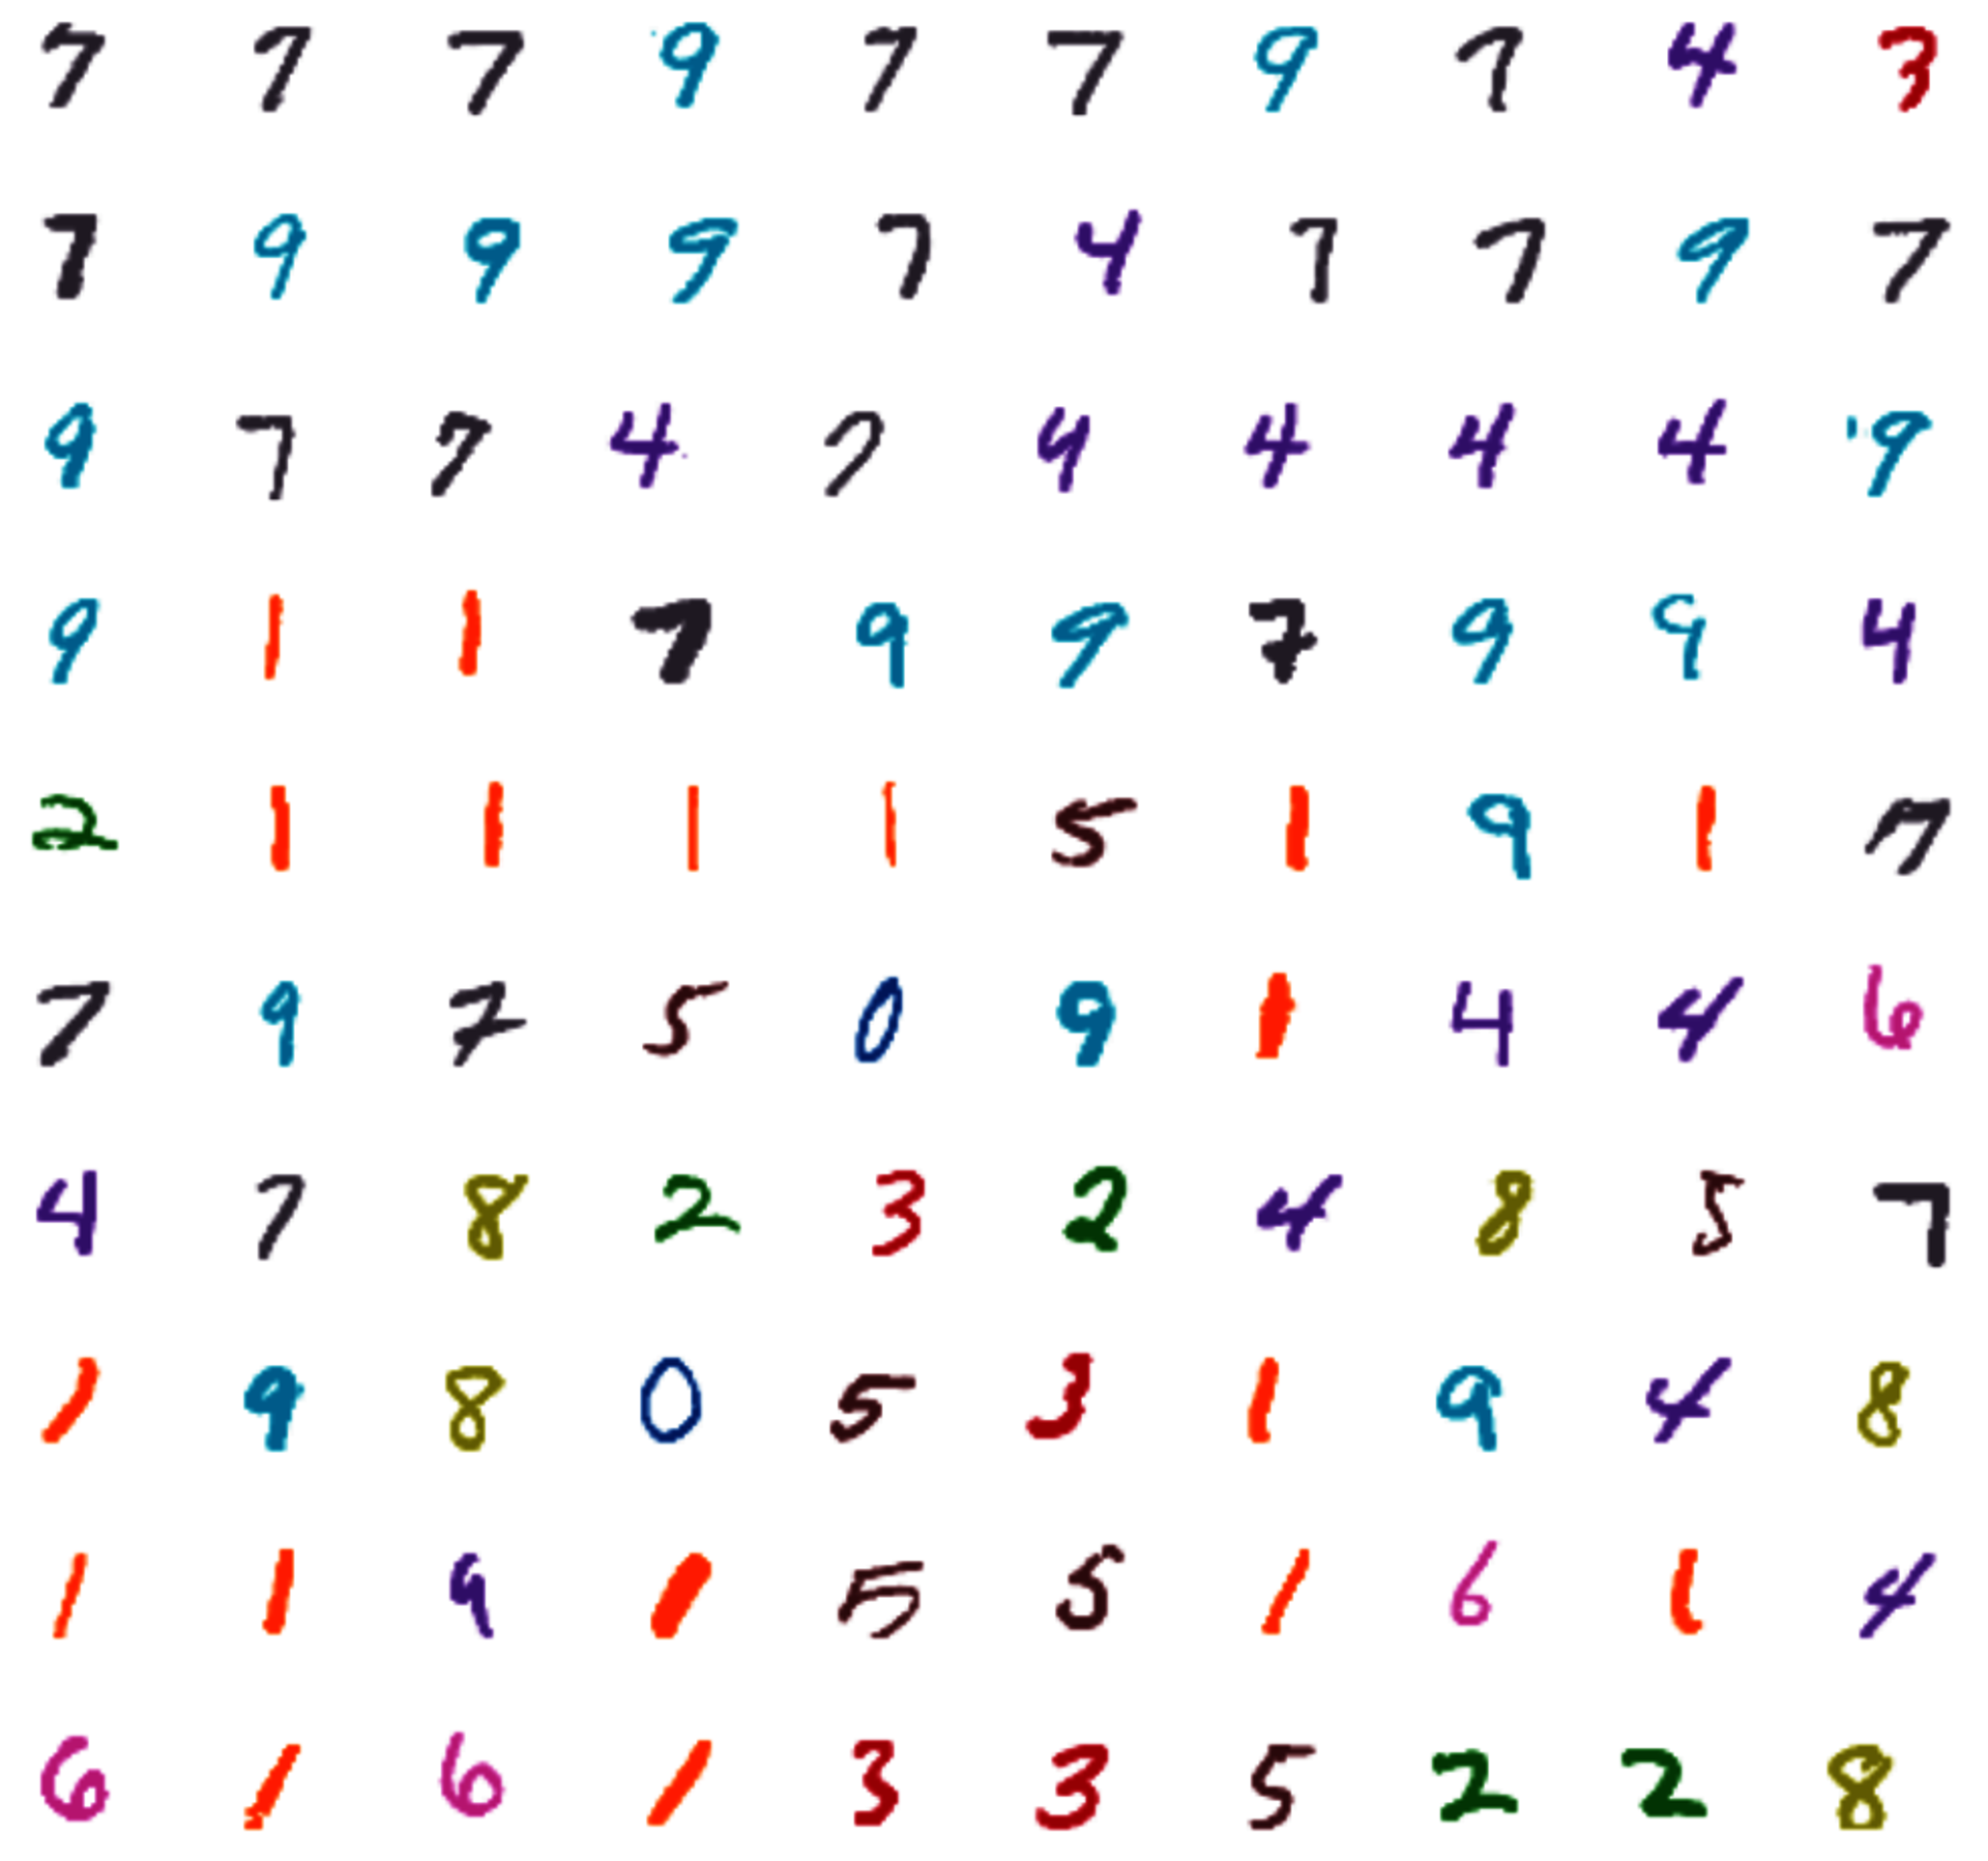
\includegraphics[width=\textwidth]{figures/mnist_raw200}}
%         \caption{Examples of hand-written digit images.}
%         \label{subfig:digit_example}
%     \end{subfigure}
%     \begin{subfigure}[c]{0.53\linewidth}
%         \frame{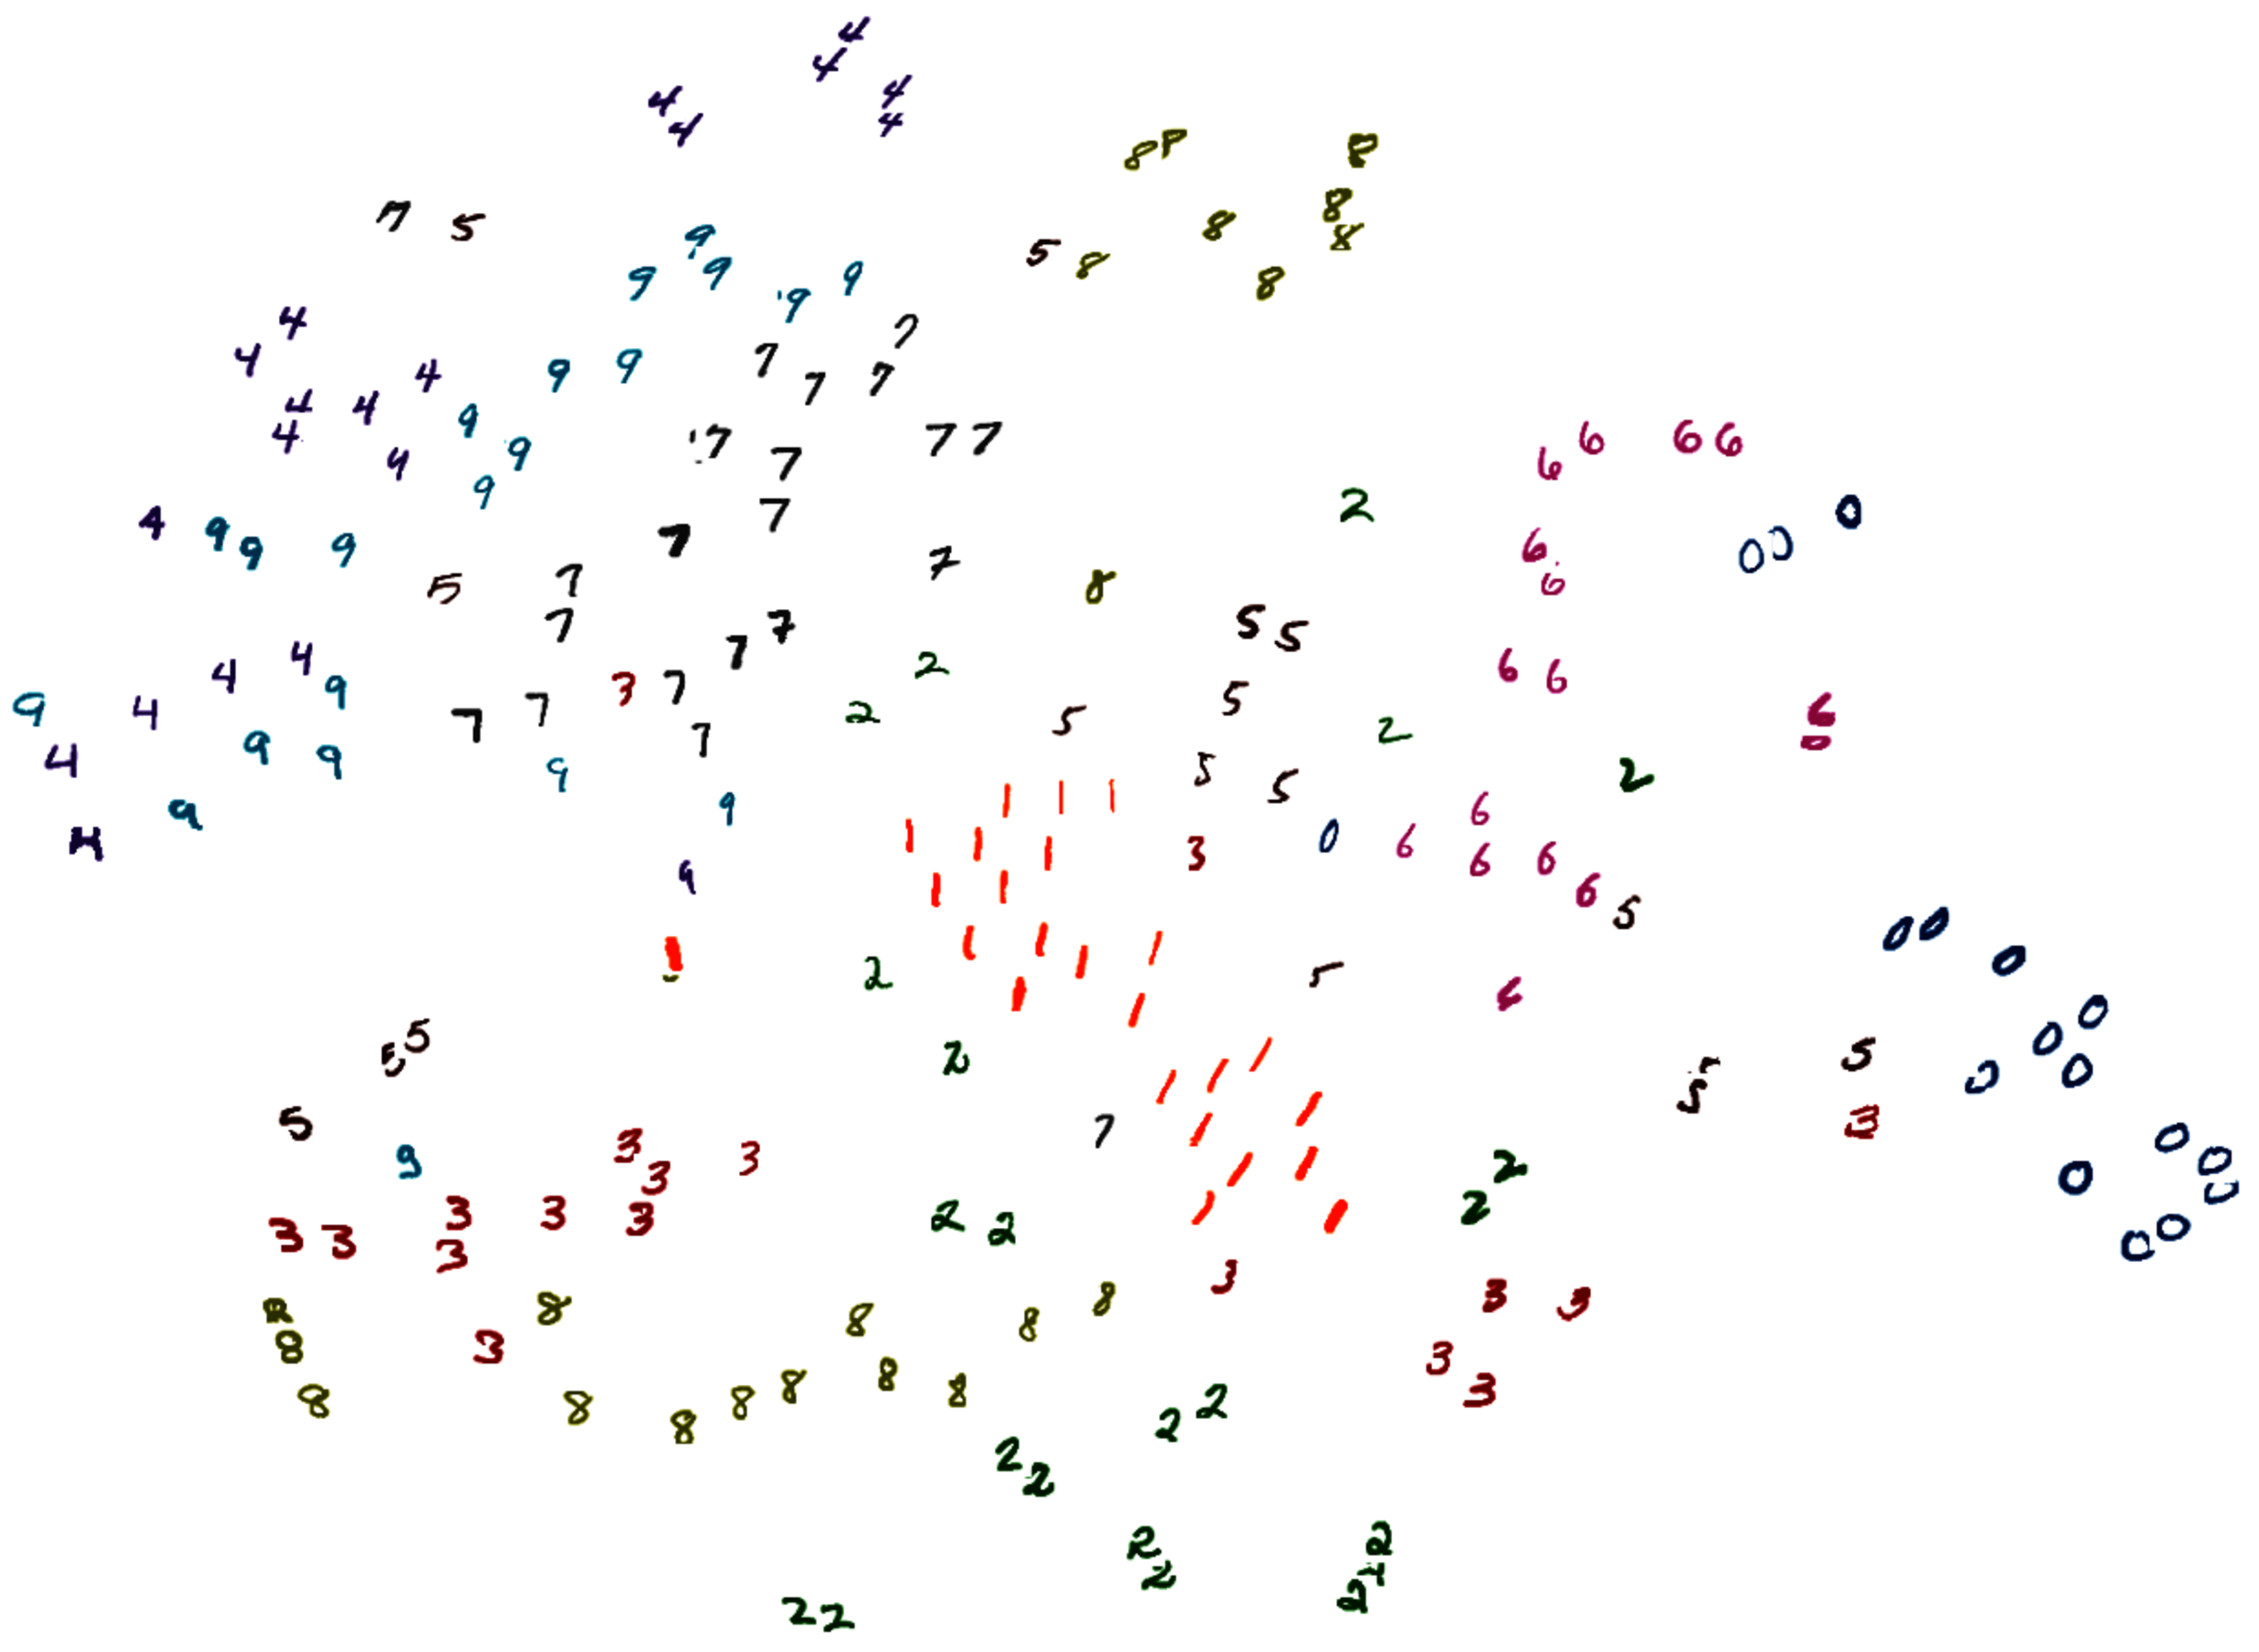
\includegraphics[width=\textwidth]{figures/mnist_viz200}}
%         \caption{A visualization created by \mbox{$t$-SNE}.}
%         \label{subfig:digit_viz_example}
%     \end{subfigure}
%     \caption{Example of 32x32 images of hand-written digits which are visualized by a dimensionality reduction technique ($t$-SNE) and represented in a 2D scatter plot.}
%     \label{fig:dr_viz}
% \end{figure}

Some DR visualization algorithms require to tune one or more hyperparameters (e.g. $t$-SNE~\cite{maaten2008tsne}, LargeVis~\cite{tang2016visualizing} and UMAP~\cite{mcinnes2018umap}). This step is crucial, since it predetermines the quality and usefulness of the obtained visualization. Typically, the desired visualization result has to be chosen through trial and error by the user among all generated results using different hyperparameter values. This process is tedious, which makes it difficult for the user to find the best suiting visualization.

\begin{figure*}%[h]
  \centering
  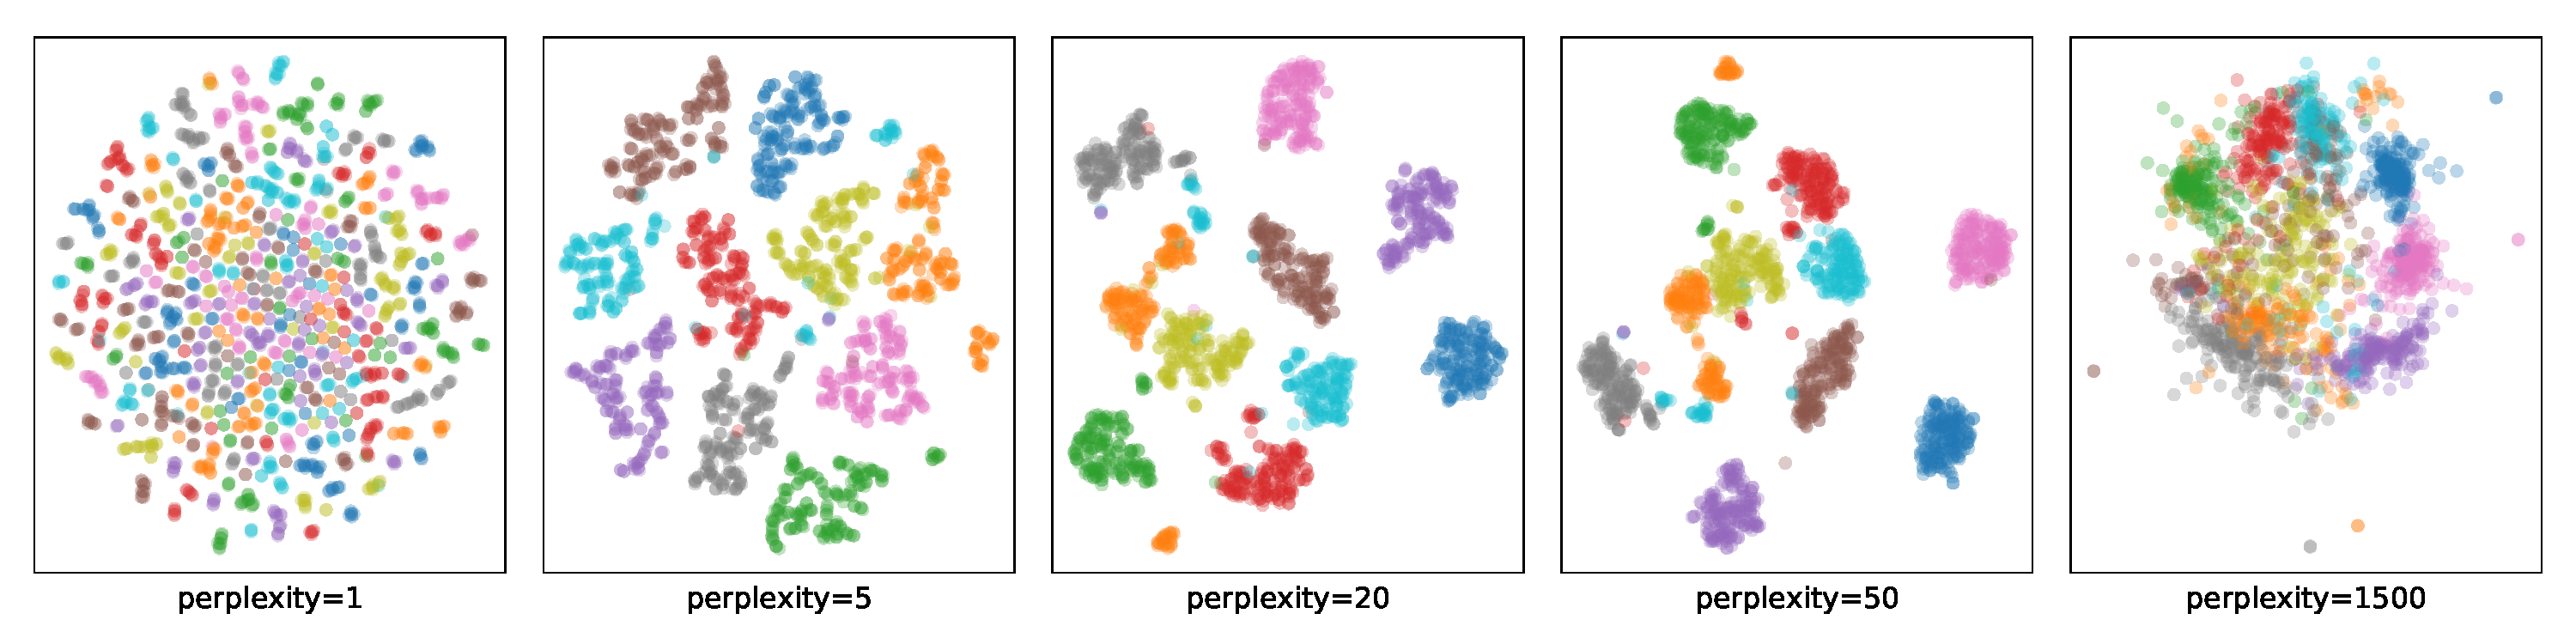
\includegraphics[width=\linewidth]{figures/MNIST-SMALL_examples}
  \caption{Visualization of the \emph{DIGITS} dataset by $t$-SNE with five different perplexity values preserving the local (left) to global (right) topology of the dataset. The dataset contains 1797 gray-scale 8x8 images representing ten different handwritten digits. The colors correspond to these different digits. Perplexities of 1 and 1500 are extreme results showing that points have one or a couple of neighbors (perplexity = 1) or they have nearly all instances in the dataset as neighbors (perplexity = 1500). Obtaining compact clusters (perplexities of 20 and 50) is usually considered better.}
  \label{fig:mnist_perps}
\end{figure*}

In this paper, we show how to automatically choose the hyperparameters of DR techniques, such as the {\it perplexity} of $t$-SNE, by considering pairwise constraints.
% We propose to consider user constraints on the dataset of interest to maximize the chance for the most suitable visualization to be presented to the user.
The constraints are in form of relationships between object pairs, which are easier to express and understand for users. These user pairwise constraints are first transformed into a quantitative measure called \emph{constraint-preserving score} and then used to find a range of hyperparameter values corresponding to the best visualizations that respect the user needs. A Bayesian optimization approach~\cite{mockus1974BO, mockus1978application} is used to find this range.

The approach of finding the best hyperparameter values with an external score, instead of modifying the chosen DR methods, allows us to apply the technique to any kind of DR methods. In that sense, the approach is DR-method-agnostic. Furthermore, our approach is a step towards the automatization of the ML pipeline (AutoML) in the context of DR, while preserving explainability. Indeed, when using the constraint for choosing the best hyperparameter values, visualizing these constraints makes it possible to explain the choice of visualization. This may ease the use of DR methods by end-users to visualizes their own data without caring about the complex algorithms and hyperparameters. Indeed, end users can use our method as a black-box hyperparameter tuning toolbox. Furthermore, the approach can also be used by DR experts to analyze the impact of hyperparameters on the quality of visualizations.

%%%%%%%% Outline of the paper
%%%%%%%%%%%%%%%%%%%%%%%%%%%%%%%%%%%%
This paper is organized as follows. Section~\ref{sec:background} presents the background on dimensionality reduction, visualization quality metrics and pairwise constraints in unsupervised learning, and provides an overview of how the automatic hyperparameter selection of DR methods is handled in the literature. Our proposed method, which takes constraints into account in order to select the best set of hyperparameter values, is introduced in Section~\ref{sec:proposed_method}. The experimental setting for evaluating our proposed method is described in Section~\ref{sec:xp:setup}. The results that are presented in Section~\ref{sec:results} and discussed in Section~\ref{sec:discussion}. Finally, Section~\ref{sec:conclusion} concludes our work.

%%%%%%%%%%%%%%%%%%%%%%%%%%%%%%%%%%%%%%%%%%%%%%%%%%%%%%%%%%%%%%%%%%%%%%%%%%%%%%%%
\section{Background and Related Work}\label{sec:background}

This section \todo[inline]{max 3 pages} presents the background and methods related to our work. Dimensionality reduction techniques that are used in our evaluation (i.e $t$-SNE, UMAP and LargeVis) are presented in Section~\ref{subsec:background_DR}. Quality measures that are used in the literature to characterize the quality of DR embeddings are presented in Section~\ref{subsec:qual_metrics_background}. The use of user constraints in clustering and in DR is presented in Section~\ref{subsec:user_constraints_clustering_DR}. Finally, the techniques to choose hyperparameters for DR algorithms are reviewed in Section~\ref{subsec:tune_HP}.%, and the way to tune it with Bayesian optimization is presented in Section~\ref{subsec:tune_with_BayOpt}.

\subsection{Dimensionality Reduction for Visualization}\label{subsec:background_DR}

Dimensionality reduction (DR) is an unsupervised learning problem in machine learning with the goal of reducing the number of dimensions of a multivariate dataset while preserving its important characteristics. In the specific case of a lower-dimensional space of two dimensions, the instances in this new space can be visualized. Typical characteristics that DR visualization techniques try to preserve are variance (as in PCA), similarities and distances between objects (distance-preserving, as in MDS), or cluster structures and neighborhood information among objects (neighborhood preservation, as in $t$-SNE) \cite{lee2007}. Three DR visualization techniques containing one or more hyperparameters are used for comparison in this paper: $t$-SNE, UMAP and LargeVis.

$t$-distributed Stochastic Neighbor Embedding ($t$-SNE)~\cite{maaten2008tsne}, one of the most widely used DR method, preserves the neighborhood information by creating an embedding in such a way that the points that are neighbors in the original high-dimensional space (HD) will still be neighbors in the reconstructed low-dimensional space (LD). 
The number of neighbors to consider for each point (controlled by the \emph{perplexity} hyperparameter) is usually determined by the user.
Fig.~\ref{fig:mnist_perps} shows some visualizations generated with different perplexities. 
It can be seen in the figure that the structure in each visualization changes according to the considered number of neighbors for each point, defined by the perplexity. When the perplexity is very small, small local groups/clusters of points appear. These groups become more and more large and compact when the perplexity increases, meaning that more neighbors for each point are preserved. However, when the perplexity is too large, each point is considered as neighbor of every other point, which leads to a crowded ball-shaped cluster. This evolution is a specific characteristic of the neighborhood-preserving DR methods. In order to use $t$-SNE efficiently, the user is required to have a good knowledge of the dataset for choosing a reasonable perplexity, as well as for interpreting and analyzing the visualization.

In the literature, the classical distance-preserving DR techniques are not always efficient because they cannot fully retain both global and local structure of the high dimensional data \cite{maaten2008tsne, van2009comparativeReview}. $t$-SNE tackles this problem by transforming the pairwise distances in HD and LD into probabilities. The intuition behind this probability-preserving approach is as follows.
Let us assume that the original data in HD is modeled by a distribution $P$ and the reduced data in LD is modeled by a distribution $Q$.
These two distributions represent the probability of being neighbors for each pair of points in HD and LD respectively.
The objective of $t$-SNE is to minimize a measure called the Kullback-Leibler (KL) divergence loss by seeking an embedding whose distribution $Q$ comes closer and closer to the true distribution $P$~\cite{maaten2008tsne}:

\begin{equation}\label{eq:p_j|i}
    p_{j|i} = \frac{\textnormal{exp}(-||x_i - x_j||^2/2\sigma_i^2)}{\sum_{k\not=i}\textnormal{exp}(-||x_i - x_k||^2/2\sigma_i^2)}
\end{equation}

\begin{equation}
    p_{ij} = \frac{p_{j|i}+p_{i|j}}{2}
\end{equation}

\begin{equation}\label{eq:q_ij}
    q_{ij} = \frac{(1+||y_i - y_j||^2)^{-1}}{\sum_{k\not=l}(1+||y_k - y_l||^2)^{-1}}
\end{equation}

\begin{equation}\label{eq:KL}
    KL(P||Q) = \sum_{i}\sum_{j} p_{ij} \textnormal{log}\frac{p_{ij}}{q_{ij}}.
\end{equation}

$t$-SNE is controlled by a hyperparameter called the perplexity, one of the most important  $t$-SNE hyperparameter, which approximates the number of neighbors considered for each point through $\sigma$ in Eq.~\ref{eq:p_j|i}. The user can change the perplexity to obtain different visualizations. With a small perplexity, the local structure is preserved, while a larger perplexity pays more attention to the global structure of the dataset. Tuning this parameter is a difficult task and is usually done by trial and error.

Uniform Manifold Approximation and Projection (UMAP) \cite{mcinnes2018umap} is a new DR technique that challenges $t$-SNE in terms of visualization quality. As for $t$-SNE, UMAP is based on a the notion of neighborhood preservation. The first phase of the algorithm is to build a weighted adjacency matrix ${\bf A}$ of a k-nearest neighbors graph in HD. The weight between the instance ${\bf x}_i$ and one of its closest neighbor ${{\bf x}_i}_j$ is defined as
\begin{equation}
    w(({\bf x}_i, {{\bf x}_i}_j)) = \textnormal{exp} \left( \frac{-\textnormal{max}(0, d({\bf x}_i, {{\bf x}_i}_j) - \rho_i)}{\sigma_i} \right),
\end{equation}
where $d(\cdot, \cdot)$ is a distance or dissimilarity measure, $\rho_i = \textnormal{min}\{d({\bf x}_i, {{\bf x}_i}_j) | 1 \leq j \leq k, d({\bf x}_i, {{\bf x}_i}_j) > 0\}$, and $\sigma_i$ is set such that
\begin{equation}
    \sum _{j=1}^k \textnormal{exp} \left( \frac{-\textnormal{max}(0, d({\bf x}_i, {{\bf x}_i}_j) - \rho_i)}{\sigma_i} \right) = \textnormal{log}_2(k).
\end{equation}
The UMAP's adjacency matrix ${\bf B}$ that is used for characterizing the HD neighborhoods is then computed as
\begin{equation}
    {\bf B} = {\bf A} + {\bf A}^\top - {\bf A} \circ {\bf A}^\top.
\end{equation}

In a second step, points ${\bf y}_i$ and ${\bf y}_j$ in LD, corresponding to HD points ${\bf x}_i$ and ${\bf x}_j$, are positioned in the 2D map according to \textit{attractive forces} defined by
\begin{equation}
    \frac{-2ab{||{\bf y}_i - {\bf y}_j||}^{2(b-1)}_2}{1+{||{\bf y}_i - {\bf y}_j||}^2_2}w(({\bf x}_i, {\bf x}_j))({\bf y}_i - {\bf y}_j)
\end{equation}
and \textit{repulsive forces} defined by
\begin{equation}
    \frac{b}{(\epsilon+{||{\bf y}_i - {\bf y}_j||}^2_2)(1+{||{\bf y}_i - {\bf y}_j||}^2_2)}(1-w(({\bf x}_i, {\bf x}_j)))({\bf y}_i - {\bf y}_j),
\end{equation}
where $a$ and $b$ are hyperparameters \cite{mcinnes2018umap}. The two hyperparameters that are considered for tuning in this paper are $k$, the number of neighbors considered, and min-dist, the distance between neighbors in LD, which is defined based on $a$ and $b$. 

The third DR visualization technique that is used in our evaluation is LargeVis. LargeVis has been developed to overcome the scalability problem that face many DR techniques. Indeed, with millions of instances, state-of-the-art techniques such as $t$-SNE does not work \cite{tang2016visualizing}. While the first step of LargeVis is to efficiently build a k-nearest neighbor graph in HD based on $t$-SNE $p_{j|i}$ (see Eq.~\ref{eq:p_j|i}), the second step is to match the probability that an edge $e_{ij}$ links the instances ${\bf x}_i$ and ${\bf x}_j$ in HD (i.e. they are neighbors) with the distance between the corresponding points ${\bf y}_i$ and ${\bf y}_j$ in LD:
\begin{equation}
    P(e_{ij}) = f(||{\bf y}_i - {\bf y}_j||),
\end{equation}
where $f$ is a probabilistic function \cite{tang2016visualizing}. With the generalization that an edge $e_{ij}$ takes a weight $w_{ij}$ defined by $P(e_{ij} = w_{ij}) = P(e_{ij} = 1)^{w_{ij}}$, LargeVis objective function becomes
\begin{equation}
    \sum_{(i,j) \in E} w_{ij}logp(e_{ij} = 1) + \sum_{(i,j) \in \bar{E}} \gamma log(1 - p(e_{ij} = 1)),
\end{equation}
where $\gamma$ is a weight given to non-existing edges. As LargeVis is based on the $p_{j|i}$ of $t$-SNE, the perplexity is also a hyperparameter of LargeVis.

%Now that the state-of-the-art DR visualization methods that contain hyperparameters are presented, metrics that can assess the quality of DR produced visualizations are reviewed and discussed in the next section.

\subsection{Visualization Quality Metrics}\label{subsec:qual_metrics_background}

There exist several metrics to evaluate the quality of an embedding.  
In this paper, clustering-based quality measures are not considered because they need labeled data for measurement (e.g. the digits in the dataset DIGITS).
%For these reasons, we only use cluster-label agnostic metrics.
We also avoid quality measures that are linked to the objective function of SNE, e.g. Neighborhood Retrieval Visualizer (NeRV) \cite{venna2010}, (i) because they need the evaluation of their own perplexity parameter and (ii) because of the bias of measuring the quality of $t$-SNE and LargeVis with a quality metric too closely related to SNE.

\begin{table}%[width=\textwidth,cols=6,pos=h]
\caption{Properties of the five cluster-label-agnostic quality metrics considered in this paper to assess visualizations.}\label{tab:metrics}
\begin{tabular}{p{1.5cm} p{0.8cm} p{4.5cm}}
\toprule
Metric name &  Range value & Description\\
\midrule
CC & $[0, 1]$ & Pearson correlation coefficient between pairwise distance vectors\\
NMS & $[0, +\infty[$ & Stress based on comparison of pairwise distance orders\\
CCA & $[0, +\infty[$ & Stress with emphasis put on LD\\
NLM & $[0, +\infty[$ & Stress with emphasis put on HD\\
AUC$_{log}$RNX & $[0, 1]$ & How neighbors in HD are preserved in LD\\
\bottomrule
\end{tabular}
\end{table}

Five metrics have been selected for evaluating the quality of visualizations. 
The first considered metric, the \emph{correlation coefficient} (CC)~\cite{geng2005}, compares the pairwise distances in the HD and LD spaces by computing the correlation between the distance vectors in HD and LD. The well-known \emph{Kruskal's non-metric stress} (NMS)~\cite{kruskal1964}, often used as objective function of non-metric multidimensional scaling, is used to compare the pairwise distance orders between the high and low-dimensional space. The \emph{curvilinear component analysis stress}~(CCA) \cite{demartines1997} is a kind of Kruskal's stress with an emphasis on the embedding pairwise distances. The metric evaluates the embedding quality by looking whether if instances in the low-dimensional space are close to each other. The \emph{Sammon's non-linear mapping stress}~(NLM)~\cite{sammon1969}, is a measure similar to CCA, but focusing on the closeness of instances in the high-dimensional space. Finally, the \emph{AUC$_{log}$RNX}~\cite{lee2015} compares the neighborhood of each instance in the high and low-dimensional spaces for all possible neighborhood sizes. Table~\ref{tab:metrics} summaries these metrics and mathematical details are provided in Appendix A. 

\subsection{User Constraints for Clustering and DR}\label{subsec:user_constraints_clustering_DR}

Clustering is a machine learning problem in which the goal is to find groups (called \emph{clusters}) of instances in the data. The constraints used in clustering methods have been well studied for a long time. User constraints can incorporate domain expertise with the goal of explicitly defining the property of the expected clusters.
The popular survey by Davidson et al.~\cite{Davidson2007surveyClt} focuses on \emph{constraint-based} and \emph{distance-based} clustering methods with instance-level constraints.
In constraint-based methods, the clusters are formed in such a way that the given constraints are preserved as much as possible, e.g. PCKMeans \cite{basu2004active} and another modified version of K-Means \cite{davidson2005clustering}. % with feasibility under different types of constraints \cite{davidson2005clustering}. %$\delta-$, $\epsilon-$ and pairwise constraints
In distance-based methods, the constraints are first used to train a distance function that is later used by a clustering algorithm (e.g. \cite{bar2003learning,xing2003distance}). %, e.g. relation component analysis as distance measure \cite{bar2003learning} and constraint metric K-Means \cite{xing2003distance}.
The pairwise constraints are first introduced in constrained K-Means by Wagstaff et al. \cite{wagstaff2001constrained}. Must-link and cannot-link constraints indicate that two instances must be in the same cluster or cannot be in the same cluster, respectively.
%A similar-link constraint suggests that two points should be close, or similar, and a dissimilar-link constraint means that two points should be far apart or dissimilar.

%\subsubsection{User Constraints for Dimensionality Reduction}\label{subsec:constraints_dr}
% TODO: link to user constraints for DR
One application of user constraints in DR methods is for visualizing data in which we can inject constraints to force the output embedding to have some expected properties.
The \emph{objective constraints} can be partial labels, as in semi-supervised LDA \cite{Sugiyama2008SELF}, or constraints on the value of features, as in bounded PCA \cite{giordani2007bpca}. 
If users can interact with the visualization result, they can give their feedback in form of instance-level \emph{subjective constraints}.
Integrating user interaction into DR methods is reviewed by Sacha et al.~\cite{Sacha2017Interaction}, and Endert et al.~\cite{Endert2017SOTA} proposes a wider survey on integrating machine learning into visual analysis.
Pairwise constraints in DR are used to attract points connected by similar-links and repulse dissimilar-link constrained points. Such constraints are used in, e.g., pairwise constraints-guided feature projection~\cite{tang2007pairwise}, semi-supervised DR~\cite{zhang2007ssdr}, graph-driven constrained DR via linear projection~\cite{davidson2009gcdr} and constrained locality preserving projections~\cite{cevikalp2008CLPP}.

The objective of this paper is to show that user-constraints can also be used for automatically tuning hyperparameters of DR methods. The next section reviews how the literature handles the choice of hyperparameter values in the context of DR methods.

\subsection{Choosing Hyperparameter Values of DR Methods}\label{subsec:tune_HP}

The value of the hyperparameter depends on the characteristics of the dataset such as the number of instances (size), the topology (structure) or the density (distribution) of instances, which makes it hard to select the best one.
Concerning $t$-SNE for instance, the original paper of van der Maaten et al. \cite{maaten2008tsne} suggests typical values between 5 and 50.
However, in practice, the embedding can change drastically between two different perplexity values. Therefore, there is no evidence to ensure that the suggested perplexities are good for all datasets.
The original paper also proposes a simple method to select a good perplexity by looking at the KL loss produced by several perplexities and choose the lowest one, since it corresponds to a well-preserved neighborhood.
However, the KL loss tends to naturally decrease when the perplexity increases \cite{cao2017automatic}, which  is confirmed by our experiments, as shown in Fig.~\ref{fig:klloss}. For this reason, it is unsuitable to use the KL loss for evaluating the embedding quality since a very high perplexity would be chosen.
In practice, users have to carefully choose a hard-to-understand perplexity to obtain a good embedding.
In addition to require an expertise in machine learning, this process is often tedious and error-prone.

\begin{figure}
    \centering
    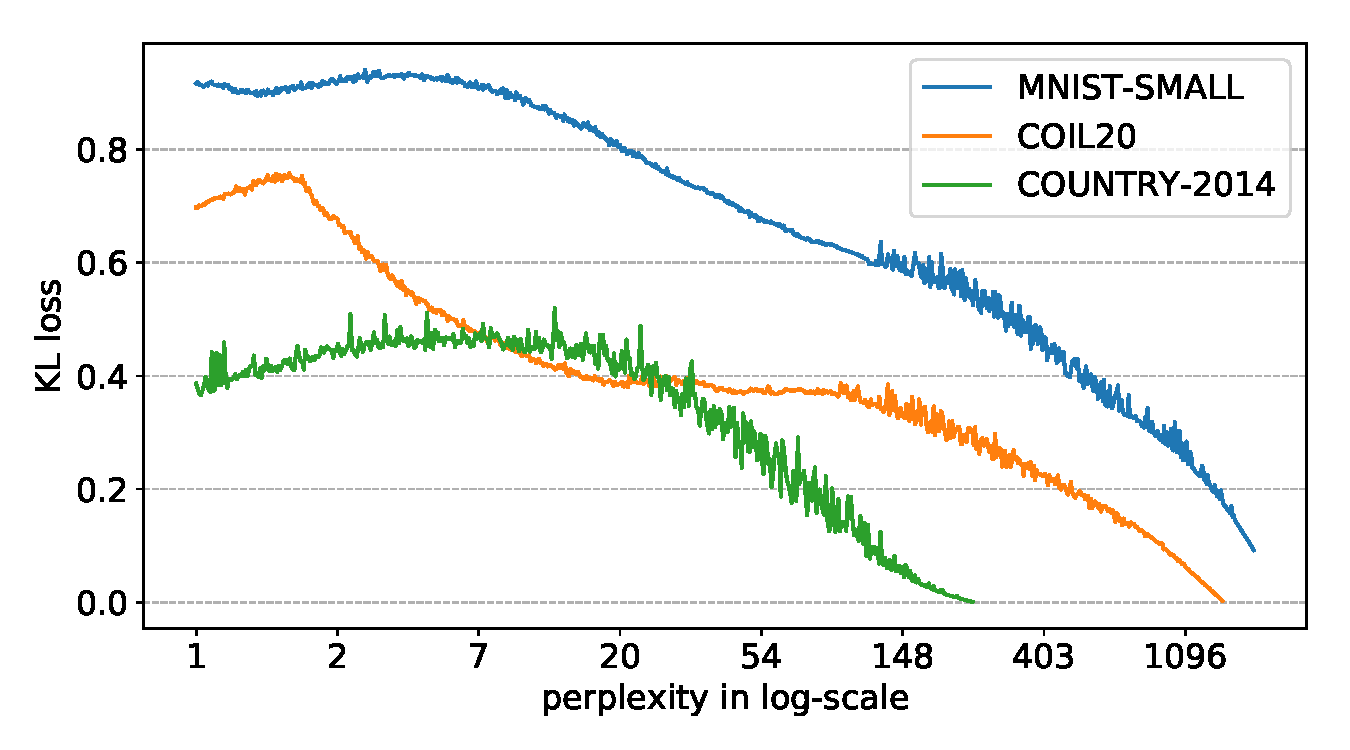
\includegraphics[width=0.95\linewidth]{klloss_all}
    \caption{For three different datasets, the KL loss tends to decrease when the perplexity increases. Note that the values of KL loss across different datasets are not comparable.}
    \label{fig:klloss}
\end{figure}

Few papers in the literature attempt to derive the best hyperparameter values automatically.
Strickert~\cite{strickert2012} avoids the burden of choosing the perplexity of $t$-SNE by evaluating the degree of neighborhood P*, instead of P, using a given pairwise score matrix S. For each instance $i$ in ${\bf S}$, all other instances $j$ are ranked and ${P}^*_{ij}$ is computed with respect to the ranking position of each instance $j$ in ${\bf S}_i$. However, this solution is not suitable when the matrix ${\bf S}$ is not provided.
Lee et al.~\cite{lee2014} use a multi-scale approach by considering, and averaging, all neighborhood sizes. Despite providing visualizations by bypassing the perplexity selection problem, these two solutions do not solve the selection problem itself.

On the contrary, Cao and Wang~\cite{cao2017automatic} try to tackle the problem by selecting the perplexity that minimizes the modified \emph{Bayesian information criteria} (BIC):
\begin{equation}
S(\textit{perplexity}) = 2KL(P||Q) + \frac{\textit{perplexity}}{n}\log(n),
\end{equation}
where $KL(P||Q)$ is the same KL loss as Eq.~\ref{eq:KL} and $n$ is the number of instances.
Their approach is validated with user-based experiments by comparing the automatically selected visualization to the ones selected by users. They obtain perplexities very close to the user consensus on three datasets. However, this method is designed only for $t$-SNE and does not make it possible to inject user knowledge through constraints.

%Bayesian methods have often been used to select hyperparameter values in supervised learning settings. Hameling~\cite{harmeling2007exploring} shows that selecting the DR visualization based on a Bayesian method can lead to good results. The next section proposes an introduction to the use of Bayesian optimization to tune DR hyperparameters.

\subsection{Hyperparameter Tuning with Bayesian Optimization}\label{subsec:tune_with_BayOpt}

% \begin{itemize}
%     \item This paper uses a Bayesian approach to find the best embedding: Exploring model selection techniques for nonlinear dimensionality reduction \cite{harmeling2007exploring}
% \end{itemize}

Machine learning methods, in general, are controlled by one or more hyperparameters.
The efficiency of a particular method is usually evaluated by a score, e.g., the F1-score for classification, V-Measure score for clustering or a visualization quality metric for DR problems.
The goal is to tune hyperparameters to
maximize the model score.
Trial-and-error is typically used to test several common combinations of hyperparameters,
but it is not the most effective way to tune them.

One common approach to solve this problem is through a naive grid search.
By making a list of discrete values for each hyperparameter,
all possible combinations can be tested.
However, the parameter space in which the search take place grows exponentially w.r.t. the number of hyperparameters
and the number of values to test for each one.
A better approach is random search \cite{bergstra2011algorithms}, in which the combinations are randomly sampled.
In this strategy, one value for each hyperparameter is picked randomly to create a combination.
However, the issue is that there are some hyperparameters that have a large effect, while some others have none.
That means checking the values for the hyperparameter that has no effect is a loss of resources.
Thus, the question is how to jointly tune many hyperparameters at the same time with as few evaluations as possible.

Bayesian optimization (BayOpt) is a strategy for finding the extremum (minimum or maximum) of an objective function $f$~\cite{mockus1974BO}.
The objective function can be any complex non-convex black-box function that does not have a closed-form expression or its derivative may not be accessible.
Finding directly the extremum of this kind of function is therefore impossible.
However, the function values, possibly noisy, can be observed for some sampled input values.
The goal of BayOpt is not to approximate the unknown objective function $f$ but instead estimate its extremum (generally speaking, its maximum) from the ensemble of observations
in form of pair of input samples and function values.
% Let define $f({\bf x}_i)$ as the observation of the target function value for the $i^{th}$ sample ${\bf x}_i$.
BayOpt constructs a statistical model describing the relationship between
the tuned hyperparameters and the target function.
Based on the pass observation, BayOpt predict the most potential hyperparameters to evaluate which should make the target function value towards its extremum.
There is a trade-off between exploration (discover the parameter space where the target function is very uncertainty) and exploitation (trying the parameter where the objective function is expected to be high).
Several strategies exist to guide the optimization process to discover the parameter space: \emph{Maximum Probability of Improvement (MPI)}, \emph{Expected Improvement (EI)}, \emph{Lower or Upper Confidence Bound (UCB, LCB)}~\cite{brochu2010tutorial}.

Moreover, Bayesian model-based optimization is intuitive: it chooses the next input values to evaluate, based on past results, in order to concentrate the search on more promising values. BayOpt has been applied successfully to the problem of hyperparameters tuning \cite{snoek2012practical} or experimental design / randomized experiments \cite{letham2019constrained}.
In supervised setting or in clustering problem where we can access the class labels, the target function is simply a metric that measures the quality of the prediction or the clustering.
However in a visualization problem, the target function for measuring the quality of the visualization is more difficult to define.

%%%%%%%%%%%%%%%%%%%%%%%%%%%%%%%%%%%%%%%%%%%%%%%%%%%%%%%%%%%%%%%%%%%%%%%%%%%%%%
\section{Constraint Preserving Score}\label{sec:proposed_method}

In this section, the proposed constraint preserving score is presented. A first visual definition is illustrated in Section~\ref{subsec:visual_def}. Then, a definition for the quantification of the score is provided in Section~\ref{subsec:s_score}.

\subsection{Visual Definition of the User Pairwise Constraints}\label{subsec:visual_def}

Since humans distinguish similar and dissimilar high-dimensional objects (e.g. comparing countries only by their name, comparing images by visual features such as the shape, color, objects in the image, etc.), they can naturally express their knowledge with pairs of instances.
In Fig.~\ref{fig:ml_cl_examples}, some examples are provided of similar-links that can be formed between objects that are very similar and only differ based on the point of view, while dissimilar-links can be formed between objects of different shapes.

\begin{figure}
    \centering
    \begin{subfigure}[c]{0.48\linewidth}
        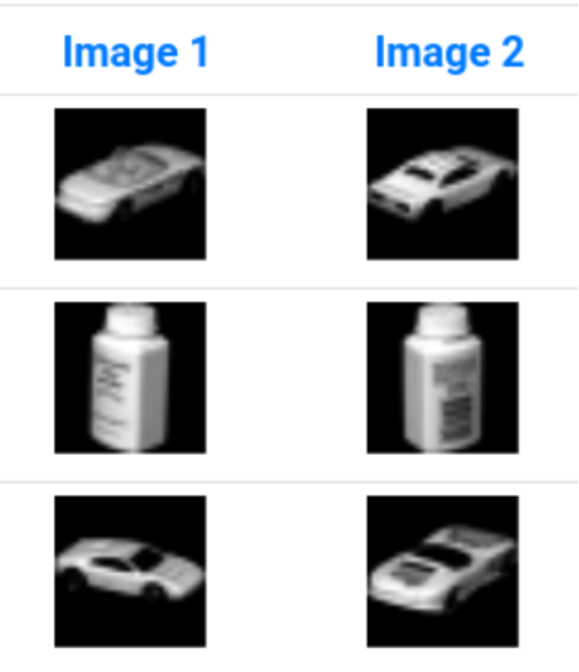
\includegraphics[width=\textwidth]{ml_examples}
        \caption{\footnotesize{Similar-link constraints.}}
    \end{subfigure}
    \begin{subfigure}[c]{0.48\linewidth}
        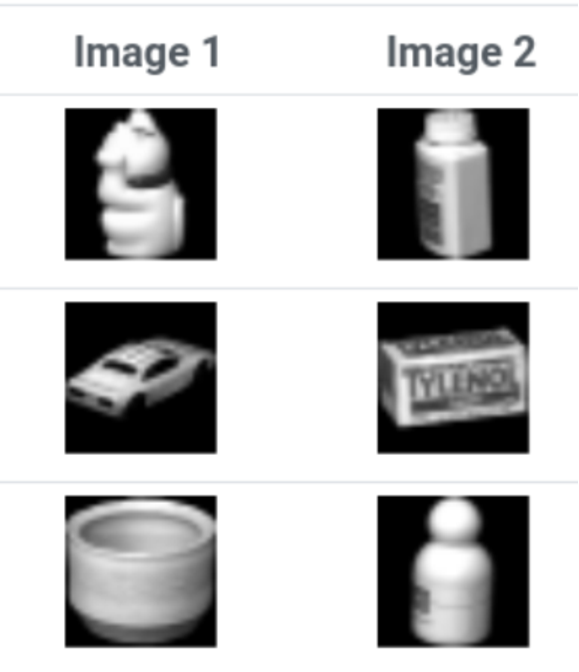
\includegraphics[width=\textwidth]{cl_examples}
        \caption{\footnotesize{Dissimilar-link constraints.}}
    \end{subfigure}
    \caption{Examples of similar-link and dissimilar-link constraints between pairs of images from COIL20 dataset (a dataset of 20 object captured under many different points of view).}
    \label{fig:ml_cl_examples}
\end{figure}

Our method is based on the hypothesis that an embedding is said to be good if it accurately represents the high-dimensional data and satisfies some given constraints.
If labels related to the dataset, which have not been used during the NLDR process, are provided, a portion of these labels can be used to generate the constraints for computing a quality score.
%This is a way to select the visualization that best fit the prior knowledge represented by the labels.
If the dataset does not contain any label, or if some particular knowledge have to be considered, constraints can directly be provided by users.
%The pairwise constraints are then used as a criterion to evaluate the fit between visualizations and user requirements. By computing this constraint score, our method makes it easier to select the NLDR hyperparameters by providing good quality embeddings that preserves the predefined constraints.

%To evaluate the reliability of the quantitative score that is derived from the pairwise constraints (defined in Section~\ref{subsec:s_score}), the score is compared with several embedding quality metrics (presented in Section~\ref{sec:result:compare}).

\subsection{Defining the Pairwise Constraints}\label{subsec:s_score}

Given a set of labeled points or user pairwise constraints, the \emph{constraint-preserving score} $f_{score}$ measures how well the pairwise constraints are preserved in a certain embedding.

\subsubsection*{Constraint Measurement}
As $t$-SNE efficiently defines links between neighboring instances, we base our constraint measurement on it. $t$-SNE uses the Student's $t$ distribution to encode the neighborhood information of the instances in the low dimensional space (see Eq.~\ref{eq:q_ij}).
The constraint-preserving score $f_{score}$ also uses a $t$ distribution in the embedded space to quantify the constraints preservation.
Let us denote the NLDR embedding result ${Y} = \{{{\bf y}_i}\}$, the set of similar-links $\mathcal{S}$ and the set of dissimilar-links $\mathcal{D}$. 
%The number of similar-link and dissimilar-link constraints are denoted by $|\mathcal{S}|$ and $|\mathcal{D}|$, respectively.
For a constrained pair of instances $({\bf y}_i, {\bf y}_j)$, the probability of ${\bf y}_i$ and ${\bf y}_j$ being neighbors is defined as
\begin{equation}\label{equ:q_link}
    q_{ij} = \frac
    { ( 1 + || {\bf y}_i - {\bf y}_j ||^2 )^{-1} }
    { \sum_{k \neq l} { ( 1 + ||{\bf y}_k - {\bf y}_l||^2 )^{-1} } }.
\end{equation}
The instances connected by a similar-link constraint are considered as neighbors and should be close in the embedding.
The instances constrained by a dissimilar-link should stay apart in the visualization, i.e. they cannot be neighbors.
Therefore, for each similar-link $({\bf y}_i, {\bf y}_j) \in \mathcal{S}$, $q_{ij}$ should be high and, inversely, $q_{ij}$ is expected to be low for each dissimilar-link $({\bf y}_i, {\bf y}_j) \in \mathcal{D}$.

\subsubsection*{Constraint-Preserving Score for Similar-Links}
The amount of similar-link information preserved in a given embedding is measured as a log-likelihood of the joint distribution of $q_{i j}$ over all similar-links $({\bf y}_i, {\bf y}_j) \in \mathcal{S}$:
\begin{equation}
f_{score}(\mathcal{S}) = \frac{1}{|\mathcal{S}|} \log \prod_{({\bf y}_i, {\bf y}_j) \in \mathcal{S}} q_{ij}
                = \frac{1}{|\mathcal{S}|} \sum_{({\bf y}_i, {\bf y}_j) \in \mathcal{S}} \log q_{ij}.
\end{equation}
If all pairs connected by similar-links are close, the log-likelihood is high and so is the $f_{score}(\mathcal{S})$.

\subsubsection*{Constraint-Preserving Score for Dissimilar-Links}
In contrast to similar-links, the probability $q_{ij}$ for each dissimilar-link $({\bf y}_i, {\bf y}_j) \in \mathcal{D}$ should be low, i.e. the log-likelihood over all dissimilar-link pairs ($\log \prod_{\mathcal{D}} q_{ij}$) must be minimized. In other words, the negative log-likelihood over all dissimilar-link constraints should be maximized. The constraint-preserving score for a set of dissimilar-links $\mathcal{D}$ is defined as
\begin{equation}
f_{score}(\mathcal{D}) = -\frac{1}{|\mathcal{D}|} \log \prod_{({\bf y}_i, {\bf y}_j) \in \mathcal{D}} q_{ij}
                = -\frac{1}{|\mathcal{D}|} \sum_{({\bf y}_i, {\bf y}_j) \in \mathcal{D}} \log q_{ij}.
\end{equation}
By maximizing $f_{score}(\mathcal{D})$, the embedding will respect the dissimilar-link constraints.
Another way to measure how well a dissimilar-link $({\bf y}_i, {\bf y}_j)$ is preserved is to use $1 - q_{ij}$. However, in practice, the value of $q_{ij}$ is very small, meaning that $1 - q_{ij}$ is close to one, which makes the log-likelihood of all dissimilar-links vanish.

\subsubsection*{Constraint-Preserving Score}

% \begin{figure}
%     \centering
%     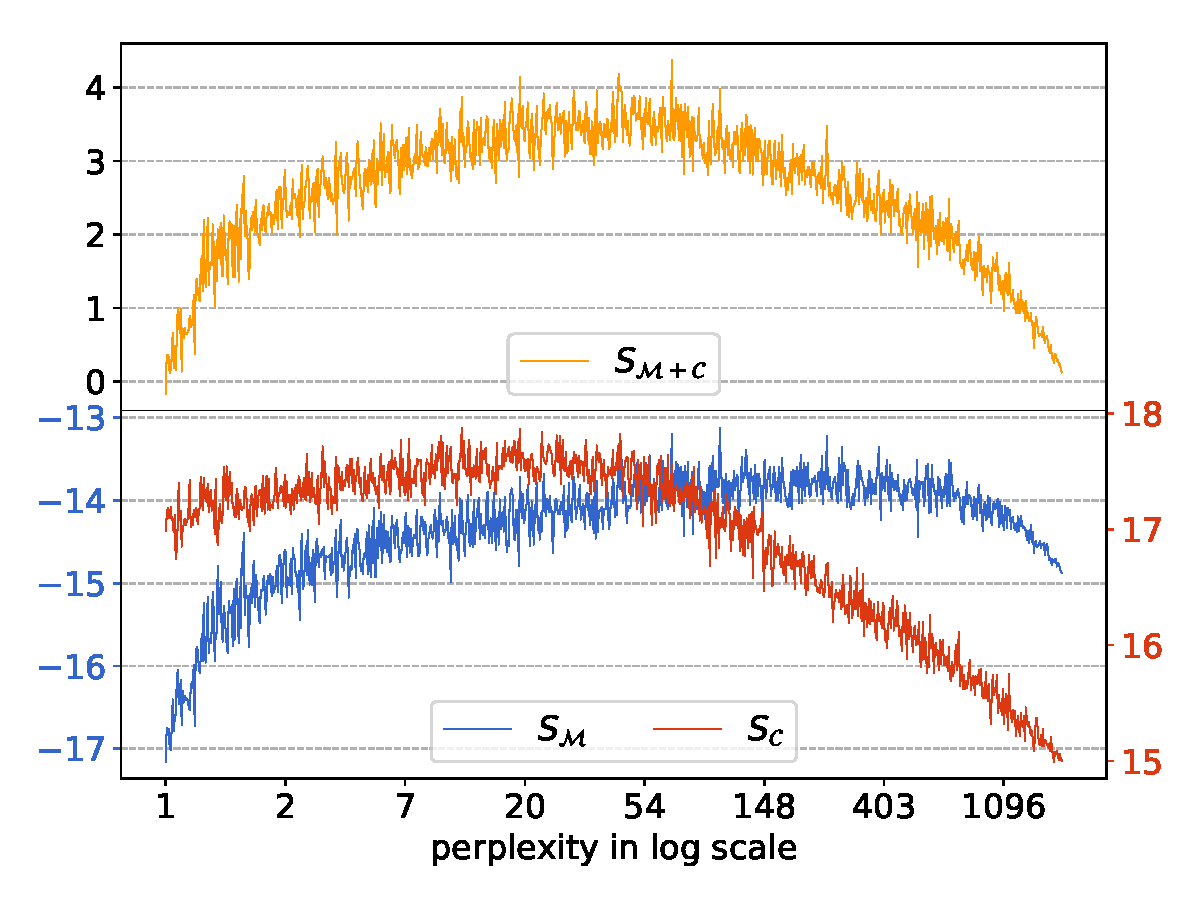
\includegraphics[width=0.85\linewidth]{s_scores_50}
%     \caption{[TODO: Replace]Evolution of constraint-preserving scores $S_{\mathcal{S}+\mathcal{D}}$, $S_{\mathcal{S}}$ and $S_{\mathcal{D}}$ with 50 constraints for $t$-SNE embeddings of \emph{DIGITS} over different perplexities.}
%     \label{fig:s_scores_mnist}
% \end{figure}

The score over all similar-constraint and dissimilar-constraint links can be defined as a combination with equal contribution of the score of both similar-links and dissimilar-links 
\begin{equation}
f_{score}(\mathcal{S},\mathcal{D}) = \frac{1}{2}f_{score}(\mathcal{S}) + \frac{1}{2}f_{score}(\mathcal{D}).
\end{equation}
$f_{score}(\mathcal{S},\mathcal{D})$ is written as $f_{score}$ for short.
An embedding that retains as much as possible the constraint information $f_{score}$ is considered to have a good quality with respect to the labels or user needs.
%Based on these definitions, our method takes a set of label- or user-defined pairwise constraints and searches, with BayOpt, among all embeddings, created by different hyperparameter values, for ones with a maximal $f_{score}$.
% Fig.~\ref{fig:s_scores_mnist} illustrates the contribution of $S_{\mathcal{S}}$ and $S_{\mathcal{D}}$ to the overall $S_{\mathcal{S}+\mathcal{D}}$ score for $t$-SNE embeddings of the \emph{DIGITS} dataset with 50 label-generated constraints (see Section~\ref{subsec:constraint_generation} for details about the generation process).

%%%%%%%%%%%%%%%%%%%%%%%%%%%%%%%%%%%%%%%%%%%%%%%%%%%%%%%%%%%%%%%%%%%%%%%%%%%%%%%%%%%%%%%%%%%%%%%
%%%%%%%%%%%%%%%%%%%%%%%%%%%%%%%%%%%%%%%%%%%%%%%%%%%%%%%%%%%%%%%%%%%%%%%%%%%%%%%%%%%%%%%%%%%%%%%
\section{Experimental Setup}\label{sec:xp:setup}

The proposed $f_{score}$ is used to find the best hyperparameters of three DR methods ($t$-SNE, LargeVis and UMAP).
This section describes the experimental setup for evaluating $f_{score}$ with six selected datasets, which are presented in Section~\ref{sec:xp:data}.
The input pairwise constraints for $f_{score}$ are presented in Section~\ref{sec:xp:constraint}.
In order to compare the proposed $f_{score}$ with other quality metrics and to evaluate the performance of the BayOpt approach, the grid of hyperparameters used and the optimization strategy for BayOpt are presented in Section~\ref{sec:xp:bo}.
%In order to compare the proposed $f_{score}$ with other quality metrics and to evaluate the performance of BayOpt approach, the grid of hyperparameters of all three DR methods are prepared and the optimization strategy for BayOpt is chosen, that are detailed in Section~\ref{sec:xp:bo}

%%%%%%%%%%%%%%%%%%%%%%%%%%%%%%%%%%%%%%%%%%%%%%%%%%%%%%%%%%%%%%%%%%%%%%%%%%%%%%%%%%%%%%%%%%%%%%%
\subsection{Experimental Datasets}\label{sec:xp:data}

\begin{table*}%[ht!]
\caption{Description of our six experimental datasets.}\label{tbl:dataset}
\begin{tabular}{m{2.2cm} m{5.4cm} m{7.4cm}}
\toprule
Dataset name & Samples & Description \\
\midrule

COIL20
    & 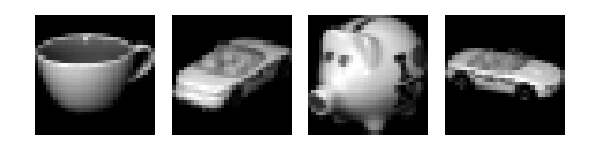
\includegraphics[width=\linewidth]{COIL20_samples}
    & 1440 gray-scale images of size 32x32, belonging to 20 classes.
    The raw images of 1024 dimensions are used directly for the DR methods.\\

DIGITS
    & 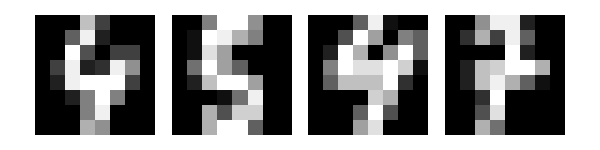
\includegraphics[width=\linewidth]{DIGITS_samples}
    & 1797 gray-scale images of size 8x8 of 10 digits.
    The raw images of 64 dimensions are used directly for the DR methods.\\

{FASHION\_1K}
    & 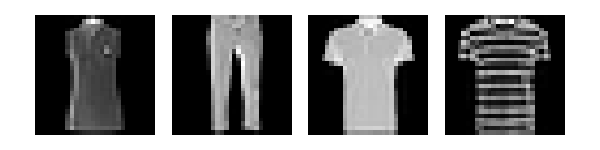
\includegraphics[width=\linewidth]{FASHION1000_samples}
    & 1000 gray-scale images of size 28x28 of 10 classes, sampled from Fashion-MNIST dataset.
    The raw images of 768 dimensions are used directly for the DR methods.\\

{FASH\_MOBI}
    & 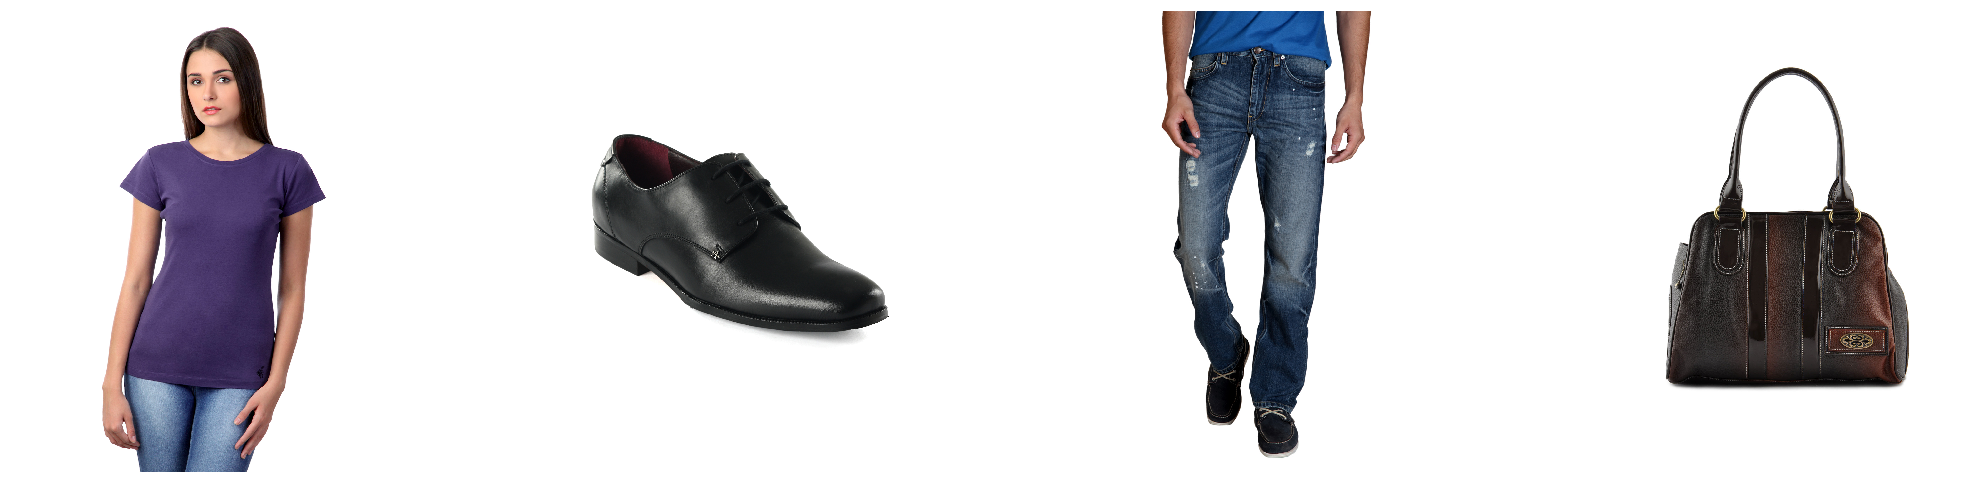
\includegraphics[width=\linewidth]{FASHION_PRODUCT_samples}
    & 1494 color images of various sizes belonging to 7 classes
    (\emph{'Bags', 'Bottomwear', 'Jewellery', 'Sandal', 'Shoes', 'Topwear', 'Watches'}),
    sampled from Fashion Product images dataset.\\

5NEWS
    & 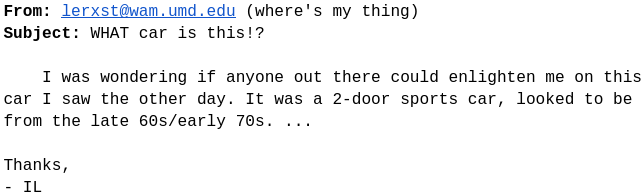
\includegraphics[width=\linewidth]{20NEWS5_samples}
    & 5 groups of 2957 emails selected from 20Newsgroups dataset,
    including \emph{'rec.autos', 'rec.sport.baseball','sci.crypt', 'sci.space', 'comp.sys.mac.hardware'}. \\

{NEURON\_1K}
    &
    & 1301 brain cells from a combined cortex, hippo-campus and sub-ventricular zone of an E18 mouse. \\

\bottomrule
\end{tabular}
\end{table*}

Six datasets of gray-scale and color images, text and gene expressions are used to evaluate our method. Table~\ref{tbl:dataset} shows a few instances for each dataset.

A first baseline dataset, DIGITS, is a subset of the optical recognition of handwritten digits dataset of 8x8 gray-scale images \cite{kaynak1995methods}.
The second baseline dataset, COIL20, is a dataset of 32x32 gray-scale images of 20 rotated objects  \cite{nene1996}.
The third baseline dataset, {FASHION\_1K}, contains 1000 28x28 gray-scale images, sampled from Fashion-MNIST clothing dataset~\cite{xiao2017/online}.
The gray-scale images from the three above datasets are normalized and used directly in the DR methods.

The first real-world image dataset, \emph{FASHION\_MOBILENET} dataset ({FASH\_MOBI} for short), contains samples of the seven most numerous classes from the fashion product images dataset~\cite{fashionproduct}.
MobileNet\cite{howard2017mobilenets} with pre-trained weights from ImageNet is used for feature extraction.
The last fully connected layer of the network is replaced by a global average pooling layer \cite{lin2013network} to obtain the flattened output vector of 1280 dimensions.
To speed up DR methods for visualization task, PCA is then applied to take only 75 features.

The second real-word dataset is a textual dataset. The 5NEWS dataset contains the text of 5 groups selected from the 20 Newsgroups dataset, which are converted to a matrix of token counts via Term Frequency Inverse Document Frequency (TF-IDF) method.
The count vectors are then fed into a Latent Dirichlet Allocation (LDA)~\cite{blei2003latent} model to extract 15 hidden topics, which are the 15 features used by the DR methods.

Our last real-world dataset is the open {NEURON\_1K} dataset~\cite{neuron1k}, which contains 1301 brain cells from an E18 mouse. These cells have been processed and provided by 10X Genomics, a company who provides chromium single cell gene expression solution and released several public genetic datasets\footnote{https://www.10xgenomics.com/resources/datasets/, the datasets are licensed under the Creative Commons Attribution license.}.
The processed data have 10 PCA features and 6 labels found by a graph-based clustering method.


%%%%%%%%%%%%%%%%%%%%%%%%%%%%%%%%%%%%%%%%%%%%%%%%%%%%%%%%%%%%%%%%%%%%%%%%%%%%%%%%%%%%%%%%%%%%%%%
\subsection{Constraint Generation}\label{sec:xp:constraint}

The input for our constraint preserving scores is an ensemble of constraints in the form of similar and dissimilar links.
% When labels are provided, they can be used to generate constraints. However, our method does not need many constraints to be stable, which means that we use a small subset of labeled instances to generate the constraints.
However, it is hard to control the quality of the constraints when they are selected manually.
For example, defining a similar link between two instances that are really different in HD may provide constraint of lower quality.
The number of constraints of each type also affects the stability of the score.
In order to correctly evaluate the score function, we use a small subset of labeled instances to generate the constraints.

Given a dataset of $C$ classes, $k$ labeled instances are randomly considered for each class.
Suppose that the number of instances in each class is larger than $k$ ($k$ is usually very small),
a similar link is formed by choosing a random pair of instances of each class.
This procedure leads to a number of similar links given by
\begin{equation}\label{eq:|S|}
    |\mathcal{S}| = {k \choose 2} C = \frac{1}{2} C k (k - 1).
\end{equation}

The dissimilar links are formed by first choosing two different classes among the $C$ classes (${C \choose 2}$ ways),
and then choosing a pair of two instances from these classes ($k^2/2$ pairs).
The number of all possible dissimilar links is therefore given by
\begin{equation}\label{eq:|D|}
    |\mathcal{D}| = {C \choose 2} \frac{k^2}{2} = \frac{1}{4} C (C - 1) k^2.
\end{equation}

% This means that the more labeled instances are considered (i.e., $k$ is larger), the more constraints are generated and the more stable the $f_{score}$ is.
% For instance, with 10 labeled instances for each of the 10 classes of the DIGITS dataset, 450 similar links and 2250 dissimilar links can be generated.
%The labeled instances are used to indicate the relationship of belonging to the same or to different groups. The points can also be freely chosen and grouped by the users to indicate the relationship they care about. The generated pairwise constraints can express the information encoded in these labeled instances. $f_{score}$ function takes the constraints as input and evaluates how well the encoded information is preserved in the embeddings. The experimental setup for proving empirically the reliability of $f_{score}$ is presented in the next section.

\subsection{Evaluation protocol}\label{sec:xp:protocol}
In order to demonstrate the characteristics of $f_{score}$ and compare it with other scores, the workflow of our experiments is as follows.
\begin{itemize}
\item First, create a grid of hyperparameters for each of the three methods ($t$-SNE, LargeVis and UMAP).
  For $t$-SNE and LargeVis, the grid is an integer vector of perplexity values in $[2,N/3]$.
  For UMAP, the two dimensional grid is created from an integer vector of {n\_neighbor} values in $[2,N/3]$ and a vector of 10 real values of {min\_dist} in $[0.001, 1.0]$.
  All hyperparameter values are sampled in natural logarithmic scale.
\item Second, calculate embedding of three DR methods for each combination of hyperparameters in the grid.
\item Third, calculate $f_{score}$, $AUC_{log}RNX$ and BIC-based score (if applicable) for each embedding.
  How to calculate $f_{score}$ and how to choose the number of input labeled instances for this score is detailed in Sec~\ref{sec:characteristics}.
  The comparison between $f_{score}$ and two other scores is detailed in Sec.~\ref{sec:compare}.
\end{itemize}

It should note that the grid of hyperparameters is only used to empirically analyze and compare the characteristics of the proposed $f_{score}$ and two other scores .
After proving that $f_{score}$ is reliable, we present how to use it in BayOpt to quickly find the best combination of hyperparameters for a given DR method in Sec~\ref{sec:apply-bayopt}.

%%%%%%%%%%%%%%%%%%%%%%%%%%%%%%%%%%%%%%%%%%%%%%%%%%%%%%%%%%%%%%%%%%%%%%%%%%%%%%%%
\section{Characteristics of $f_{score}$}\label{sec:characteristics}

The proposed constraint preserving score is a function of the pairwise constraints, which can be generated automatically from input labeled instances.
Through the experiments, we show that $f_{score}$ is a \emph{well behaviored} \todo[inline]{explain more convex-like} function which has three following important characteristics.
It is stable w.r.t. the number of input labeled instances (Sec.~\ref{sec:stability}).
It is computational efficient (Sec.~\ref{sec:efficiency}).
It is flexible w.r.t different set of input constraints (Sec.~\ref{sec:flexibility}).


\subsection{Stability}\label{sec:stability}

%% FIGURE score stability
\begin{figure}[ht!]
    \begin{subfigure}[b]{0.32\linewidth}
         \centering
         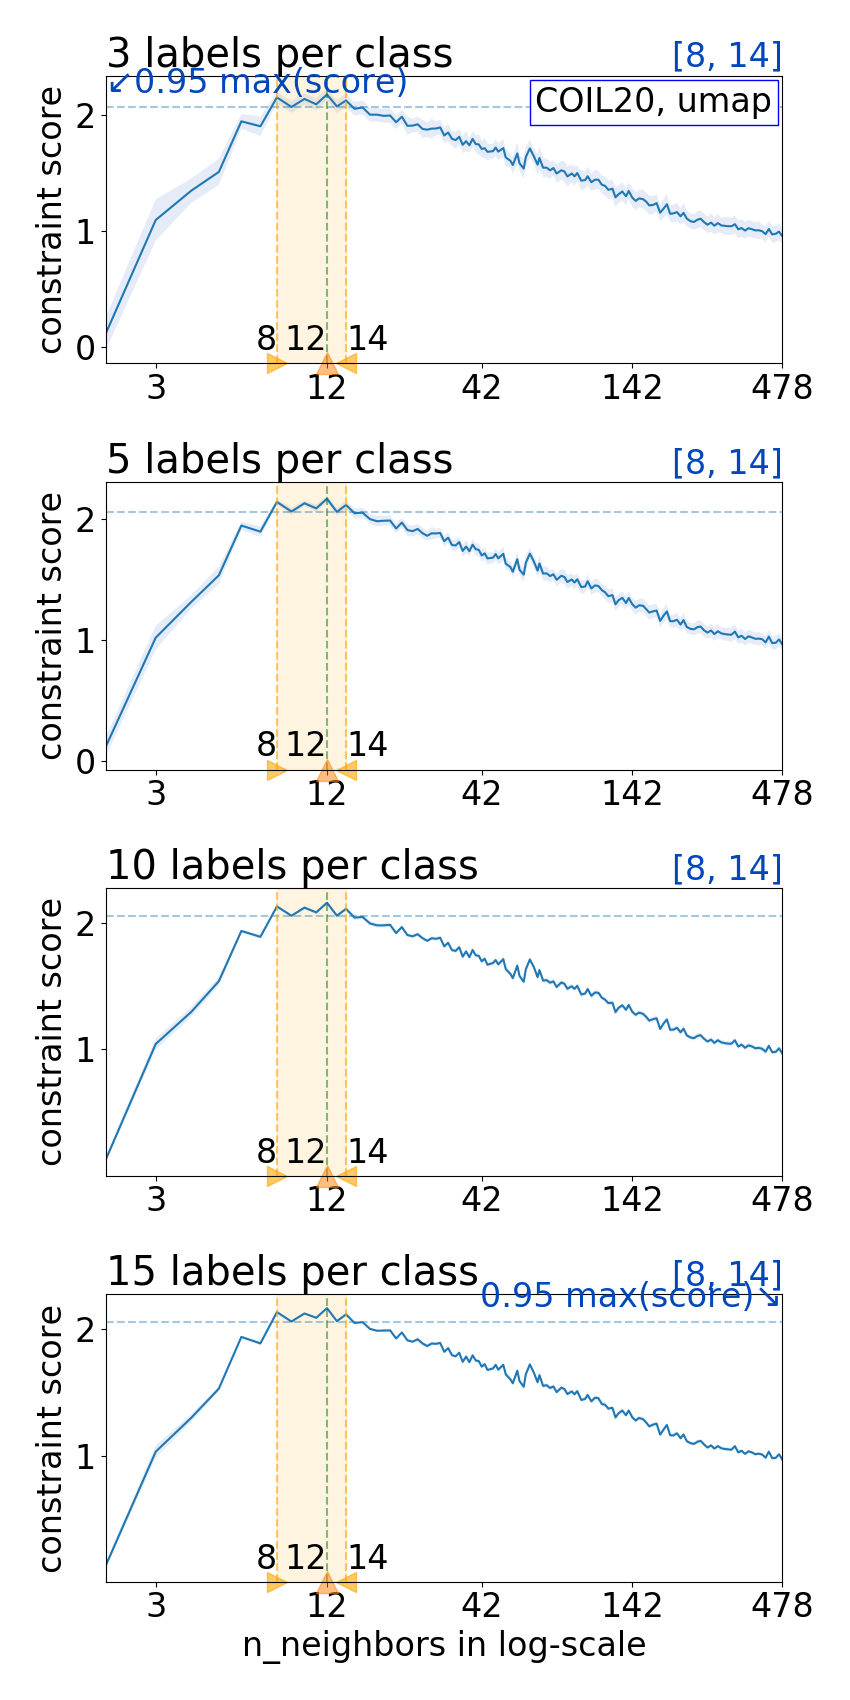
\includegraphics[width=\linewidth]{COIL20_umap_scores}
         \caption{UMAP}
    \end{subfigure}
    \hfill
    \begin{subfigure}[b]{0.32\linewidth}
         \centering
         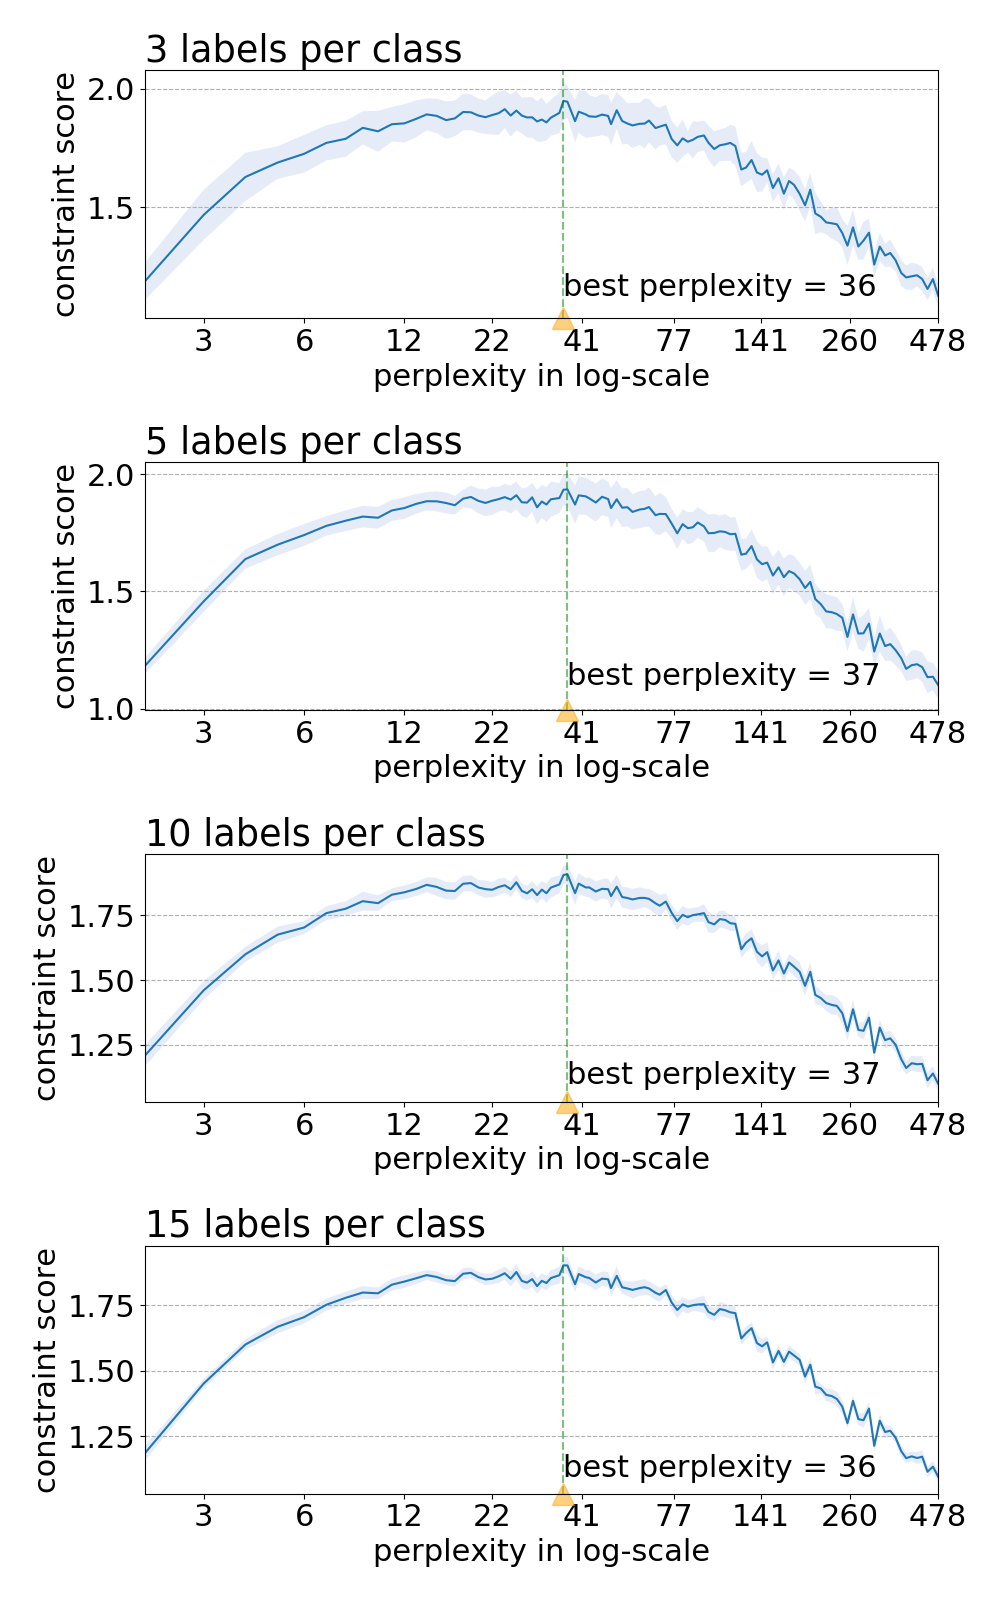
\includegraphics[width=\linewidth]{COIL20_tsne_scores}
         \caption{$t$-SNE}
    \end{subfigure}
    \hfill
    \begin{subfigure}[b]{0.32\linewidth}
         \centering
         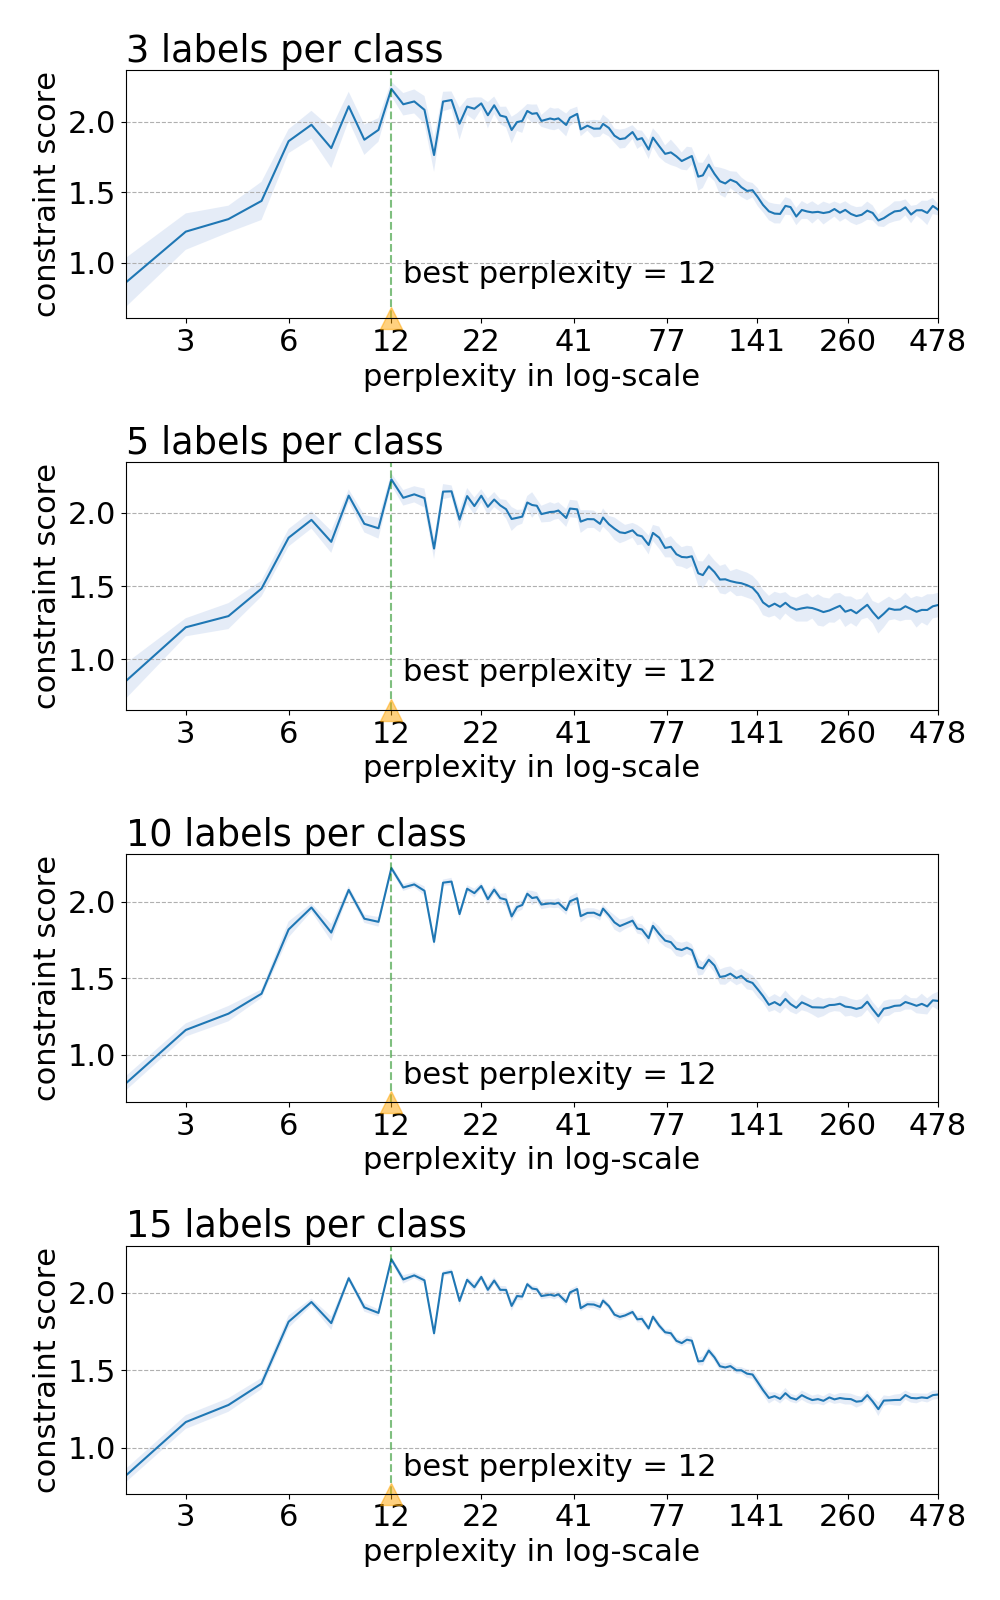
\includegraphics[width=\linewidth]{COIL20_largevis_scores}
         \caption{LargeVis}
    \end{subfigure}
    \caption{Stability of the constraint preserving scores with UMAP, $t$-SNE and LargeVis for COIL20 dataset.
    The filled region highlights the best range of hyperparameters which make the score value superior to 96\% of maximum score value.}
    \label{fig:score:stability:COIL20}
\end{figure}

We evaluate $f_{score}$ with five different numbers of labeled instances (3, 5, 10 and 15) per class.
The labeled instances are independent and not accumulated, i.e., the set of labeled instances in a setting does not contain ones of the previous setting.
In each setting, $f_{score}$ is repeatedly evaluated 20 times with different set of pairwise constraints generated from the same fixed number of input labeled instances.
Average value of $f_{score}$ for $t$-SNE, LargeVis and UMAP (with fixed {min\_dist} of 0.1) embeddings of COIL20 dataset is plotted in Fig.~\ref{fig:score:stability:COIL20}.
When the number of labeled instances increases, $f_{score}$ is more stable since the variance (presented by filled regions around the $f_{score}$ curve in the plot) decreases.
This result is shown for COIL20, but also true for the other selected datasets.

Selecting the best hyperparameter value corresponding to the maximum score may not be the best choice, since several hyperparameter values can give almost the same $f_{score}$.
We propose to evaluate a range of hyperparameter values in which $f_{score}$ has larger value than a certain threshold. % sepcific threshold
For instance, the threshold can be 96\% of the maximum $f_{score}$ value.
The best hyperparameter ranges highlighted by the vertical regions in Fig.~\ref{fig:score:stability:COIL20} are sensibly the same for the different numbers of labeled instances per label.

In summary, $f_{score}$ is stable w.r.t the number of input labeled instances.
From now on, we use 10 labeled instances per class to calculate $f_{score}$ in all experiments since it is a reasonable small number of labels and the variance of score value is negligible.


\subsection{Computational efficiency}\label{sec:efficiency}
$f_{score}$ requires an extra amount of labeled data but the computation is simple and efficient.
$f_{score}$ has a complexity of $O(N^2)$ since it only requires access to the pairwise distance between embedded points.
Furthermore, the summation over all input pairwise constraints is trivial and efficiently vectorized via matrix slicing operation.
In contrast, $AUC_{log}RNX$ must access to both HD data and the embedding.
It has a high complexity of $O(DN^2logN)$ and may not be applicable for large dataset.
The BIC-based score, despite its simplicity, can only be used for $t$-SNE.
If we force to use BIC-based score for the embedding not generated by $t$-SNE, it requires to compute $t$-SNE's KL loss, which involves the HD data and has a complexity of $O(DN^2)$.
The proposed constraint preserving $f_{score}$ is agnostic w.r.t. the DR method and computationally more efficient than both two other scores in general.


\subsection{Flexibility}\label{sec:flexibility}

%% FIGURE Score flexibility
\begin{figure*}[ht!]
    \centering
    \begin{subfigure}[b]{.32\linewidth}
        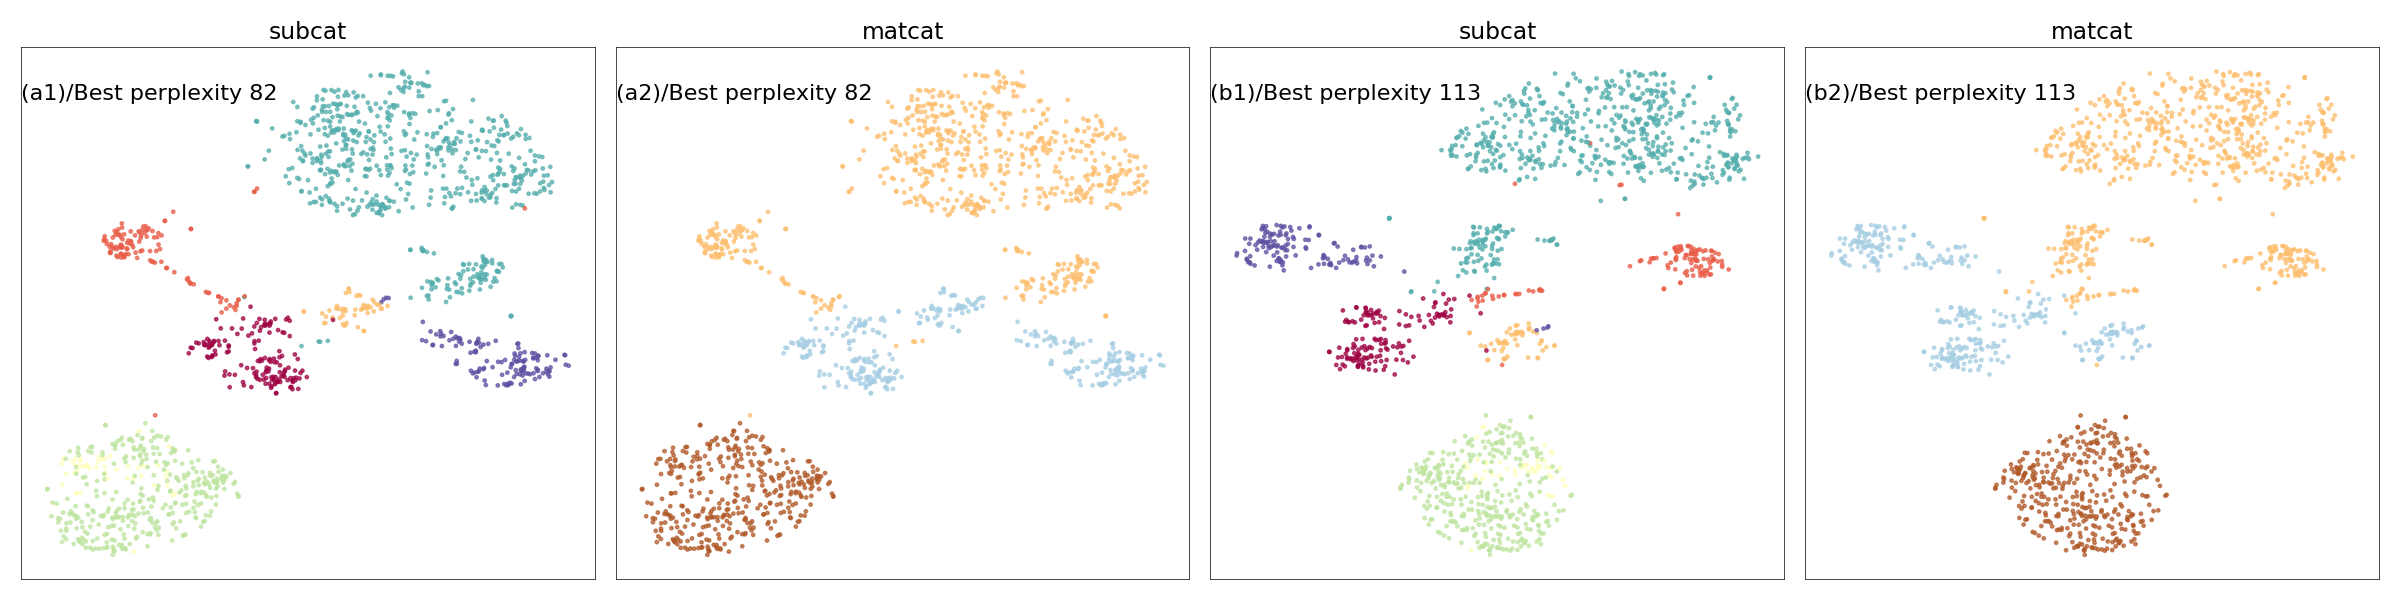
\includegraphics[width=\linewidth]{FASHION_MOBILENET_score_flexibility}
        \caption{{FASH\_MOBI} dataset}
        \label{fig:flexibility:FASHMOBI}
    \end{subfigure}
    ~
    \begin{subfigure}[b]{.32\linewidth}
        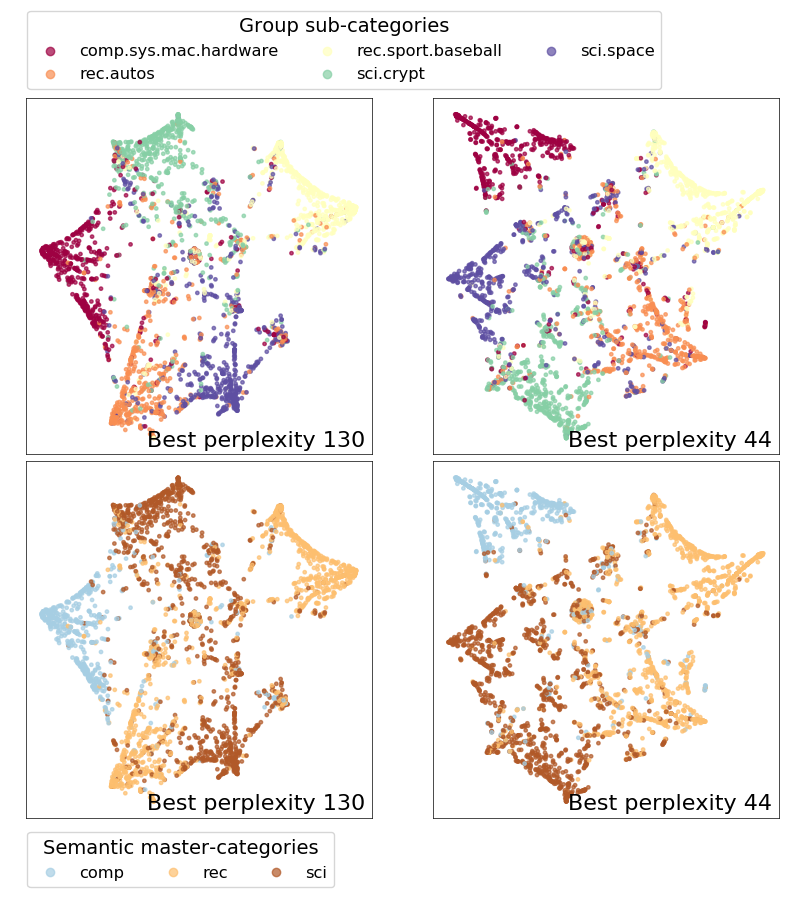
\includegraphics[width=\linewidth]{20NEWS5_score_flexibility}
        \caption{5NEWS dataset}
        \label{fig:flexibility:5NEWS}
    \end{subfigure}
    ~
    \begin{subfigure}[b]{.32\linewidth}
        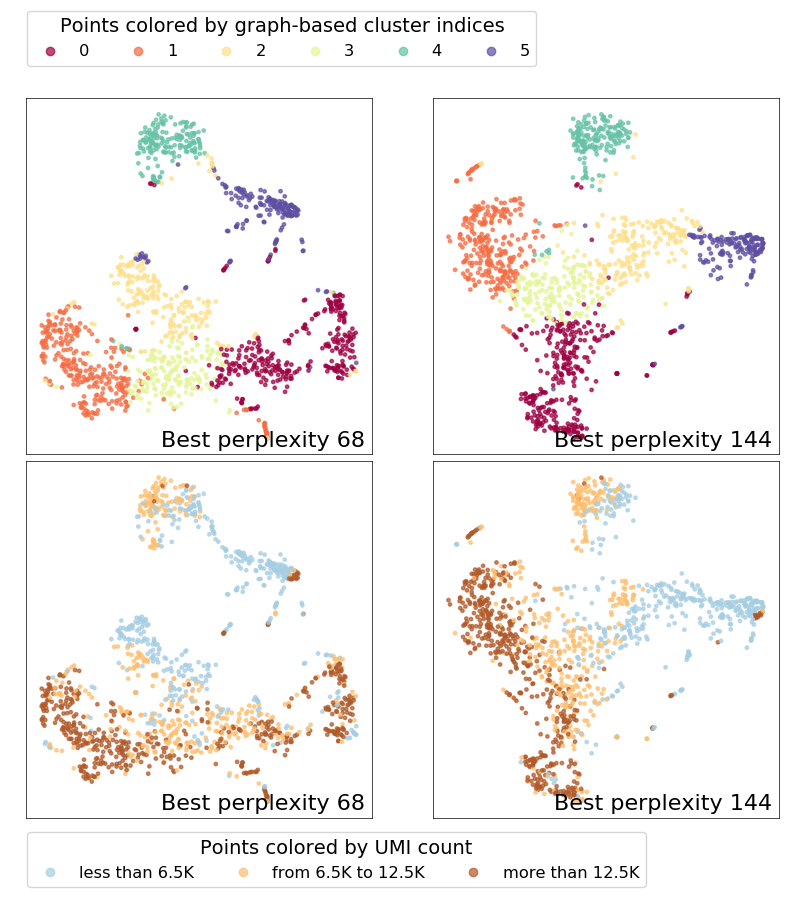
\includegraphics[width=\linewidth]{NEURON_1K_score_flexibility}
        \caption{{NEURON\_1K} dataset}
        \label{fig:flexibility:NEURON1K}
    \end{subfigure}
    ~
    \caption{Flexibility of $f_{score}$.}
    \label{fig:flexibility}
\end{figure*}

All the visualization quality metrics presented in Section~\ref{subsec:qual_metrics_background} and the BIC-based score produce a deterministic measurement since the characteristics measured by them are fixed.
In contrast, $f_{score}$ is a function of given constraints and evaluates how well these constraints are preserved.
It can measure the embeddings differently, depending on the relation encoded in the given input constraints.
The quality measurement of $f_{score}$ is therefore flexible w.r.t. to the input constraints.
For example, the constraints generated from class labels reflect naturally the class-relationship between the instances.
However, if the users want to see different pattern in the data, they can specify different constraints in $f_{score}$ to describe what they need.

Concrete examples with $t$-SNE embeddings for three real world datasets are presented in this section.
We always use 10 labeled instances per each class/group to generate pairwise constraints for $f_{score}$.

The first example is provided for {FASH\_MOBI} with seven sub-groups: \emph{'Bags', 'Bottomwear', 'Jewellery', 'Sandal', 'Shoes', 'Topwear'} and \emph{'Watches'}.
The best visualization (perplexity of 82) presents seven detached sub-groups as shown in the top-left plot of Fig~\ref{fig:flexibility:FASHMOBI}.
If the use wants to see the hierarchical grouping, they can provide the constraints in which, for example, \emph{'Bag', 'Jewellery', 'Watches'} are grouped as \emph{'Accessories'}.
\emph{'Sandal', 'Shoes'} are grouped into \emph{'Footware'}.
\emph{'Topwear', 'Bottomware'} are grouped into \emph{'Apparel'}.
The previously-chosen visualization does not reveal these three hierarchical groups.
The new best perplexity is 113, which better reveal the hierarchical structure as shown in the bottom-right corner of Fig~\ref{fig:flexibility:FASHMOBI}.

The second example concerns semantic labels for the textual 5NEWS dataset.
The five original classes can be regrouped into three more general topics.
\emph{'rec.autos', 'rec.sport.baseball'} are grouped into sportive records (\emph{'rec'}).
\emph{'sci.space', 'sci.crypt'} are grouped into a scientific group (\emph{'sci'}).
\emph{'comp.sys.mac.hardware'} stays alone in its own group (\emph{'comp'}).
The problem of the visualization found with the original constraints from class labels is that, the global structure is not always revealed: two sub-groups of the same topic can be placed far apart (bottom-left of Fig.~\ref{fig:flexibility:5NEWS}).
By using the constraints generated from labeled points of three new semantic groups, $f_{score}$ find a better visualization in which semantic groups are placed close to each other (bottom-right of Fig.~\ref{fig:flexibility:5NEWS}).

The last example is for the genetic dataset NEURON\_1K.
The original 1301 cells are grouped into 6 classes found by a graph-based clustering algorithm.
These classes are characterized by the transcriptome profiles of individual cells (presented in the RNA sequences).
However, another important aspect to characterize individual cells is the count of absolute numbers of molecules: the unique molecular identifier (UMI)~\cite{kivioja2011counting}. 
The cells are regrouped into three new groups: having less than 6.5K molecules, having from 6.5K to 12.5K molecules and having more than 12.5K molecules.
Fig.~\ref{fig:flexibility:NEURON1K} illustrates the new visualization found by $f_{score}$ with the new constraints.
It should be noted that this optimal perplexity w.r.t. the \emph{UMI count} is never discovered by neither $AUC_{log}RNX$ nor the BIC-based score.

%%%%%%%%%%%%%%%%%%%%%%%%%%%%%%%%%%%%%%%%%%%%%%%%%%%%%%%%%%%%%%%%%%%%%%%%%%%%%%%%
\section{Comparison with other scores}\label{sec:compare}

%% FIGURE metamap tSNE example
\begin{figure*}[ht!]
    \centering
    \begin{subfigure}[b]{.8\linewidth}
        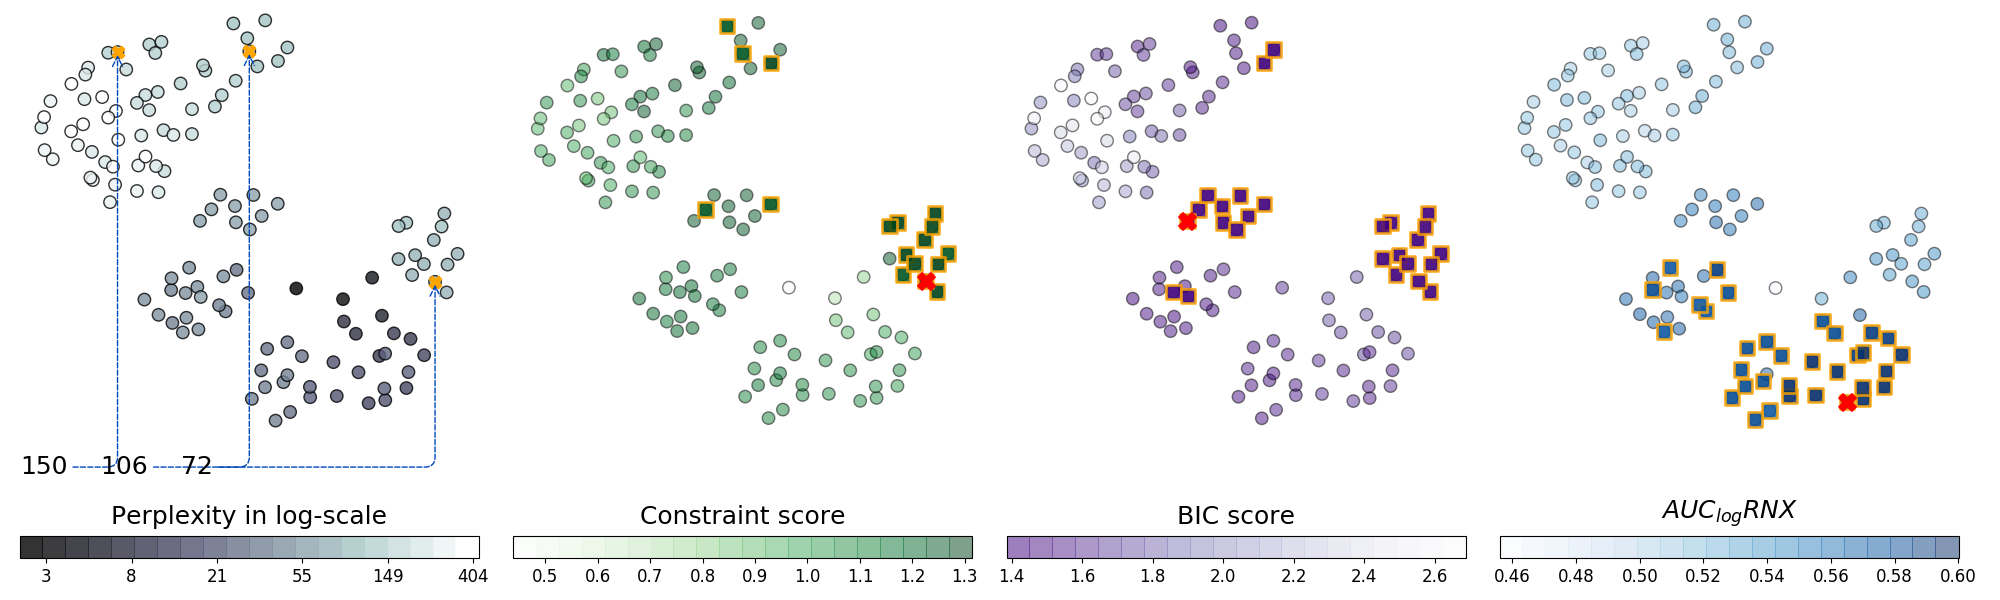
\includegraphics[width=\linewidth]{NEURON_1K_tsne_metamap}
    \end{subfigure}
    ~
    \begin{subfigure}[b]{.8\linewidth}
        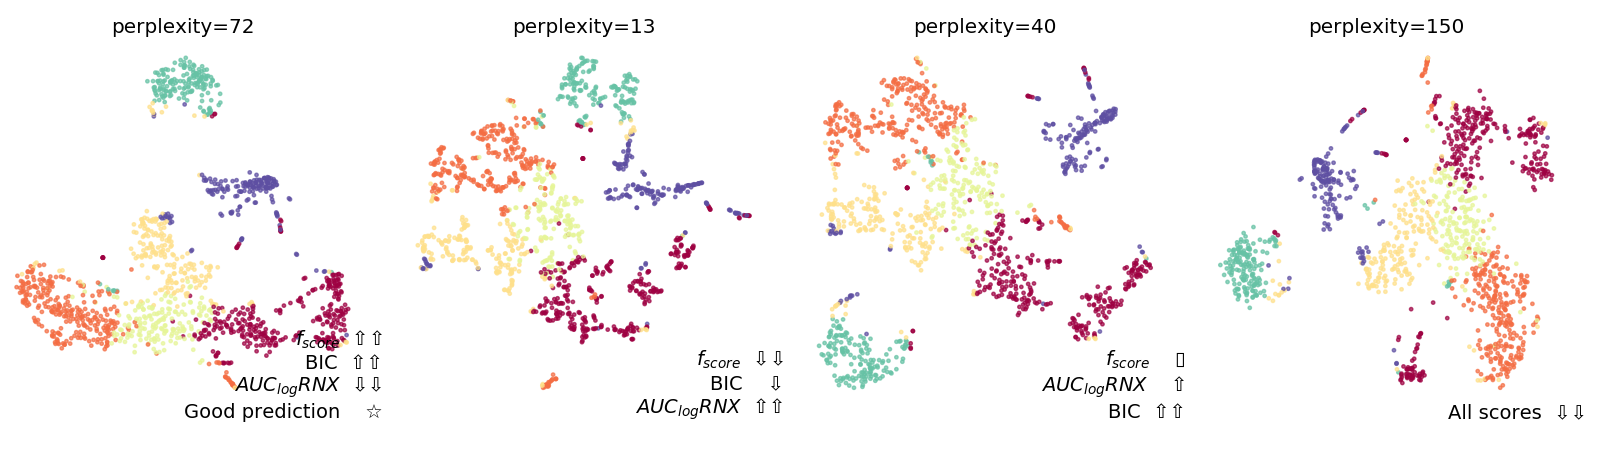
\includegraphics[width=\linewidth]{NEURON_1K_tsne_show}
    \end{subfigure}
    \caption{Metamap and sample visualizations for the selected parameters for {NEURON\_1K} dataset.}
    \label{fig:tsne:meta:NEURON1K}
\end{figure*}
~
%% FIGURE compare 3 scores tSNE
\begin{figure}[ht!]
    \centering
    \begin{subfigure}[b]{0.3\linewidth}
        \centering
        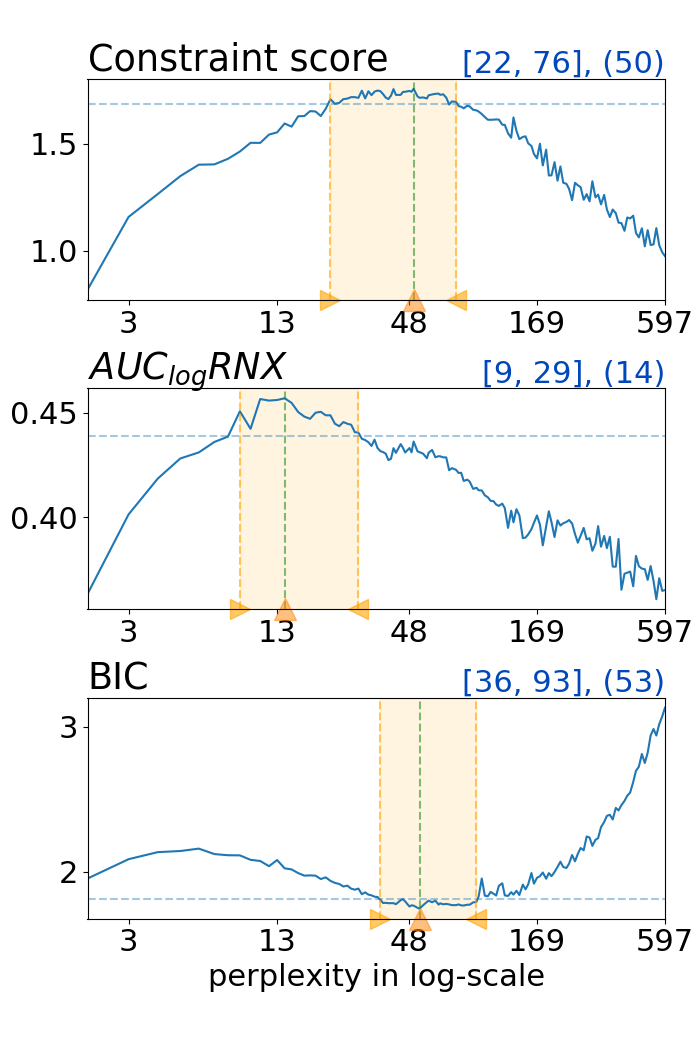
\includegraphics[width=\linewidth]{DIGITS_tsne_compare_scores}
        \caption{DIGITS}
    \end{subfigure}
    ~
    \begin{subfigure}[b]{0.3\linewidth}
        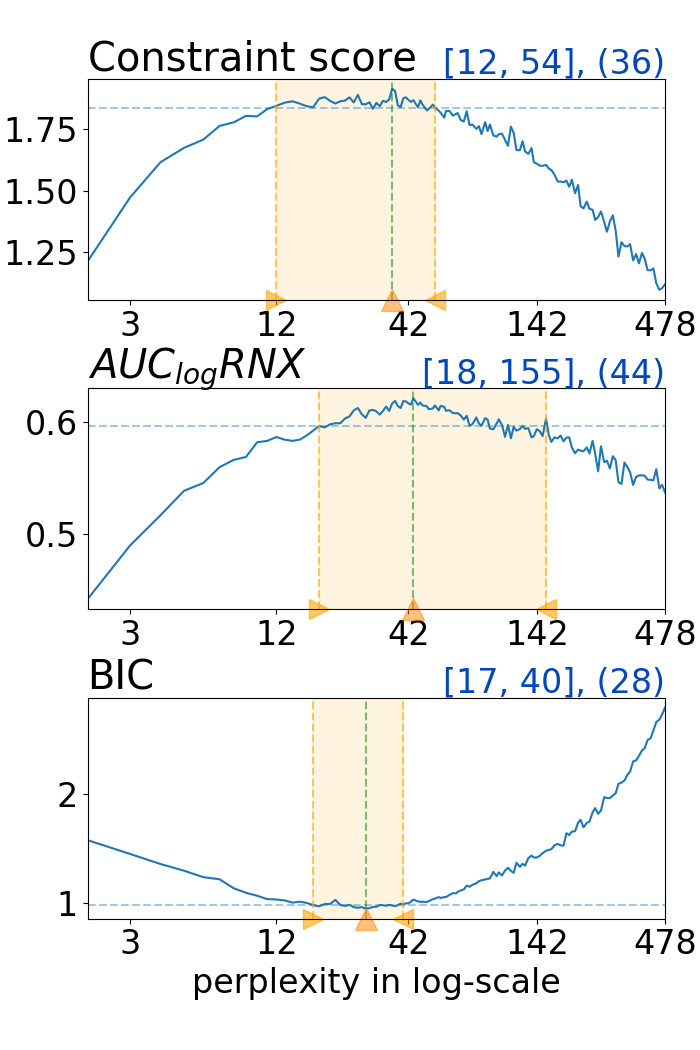
\includegraphics[width=\linewidth]{COIL20_tsne_compare_scores}
        \caption{COIL20}
    \end{subfigure}
    ~
    \begin{subfigure}[b]{0.3\linewidth}
        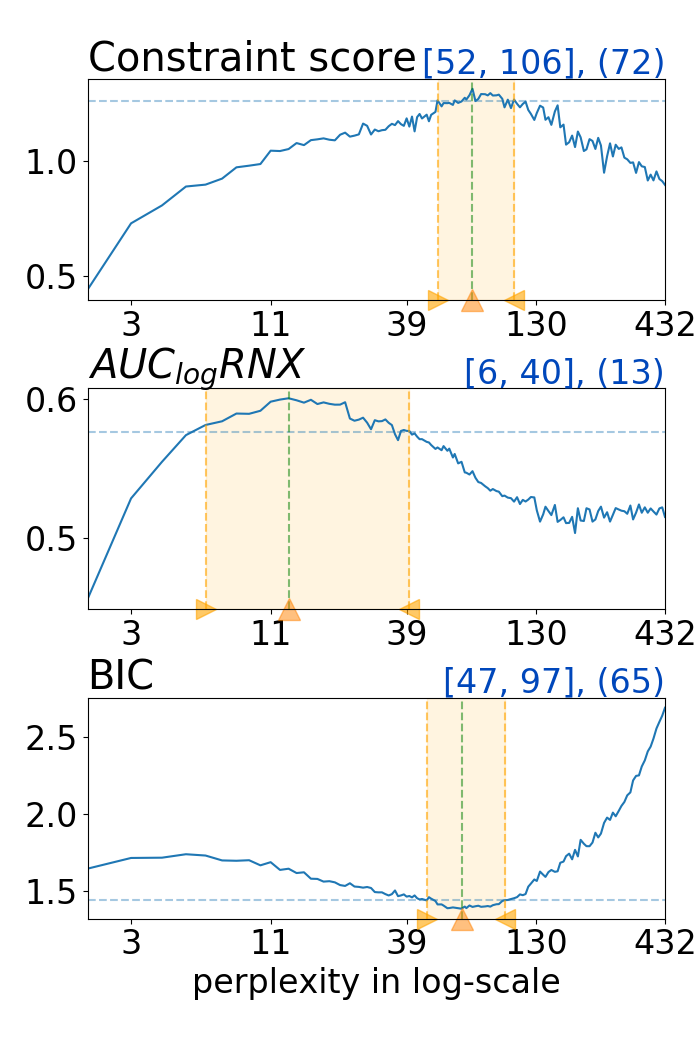
\includegraphics[width=\linewidth]{NEURON_1K_tsne_compare_scores}
        \caption{NEURON\_1K}
    \end{subfigure}
    \vfill
    \begin{subfigure}[b]{0.3\linewidth}
        \centering
        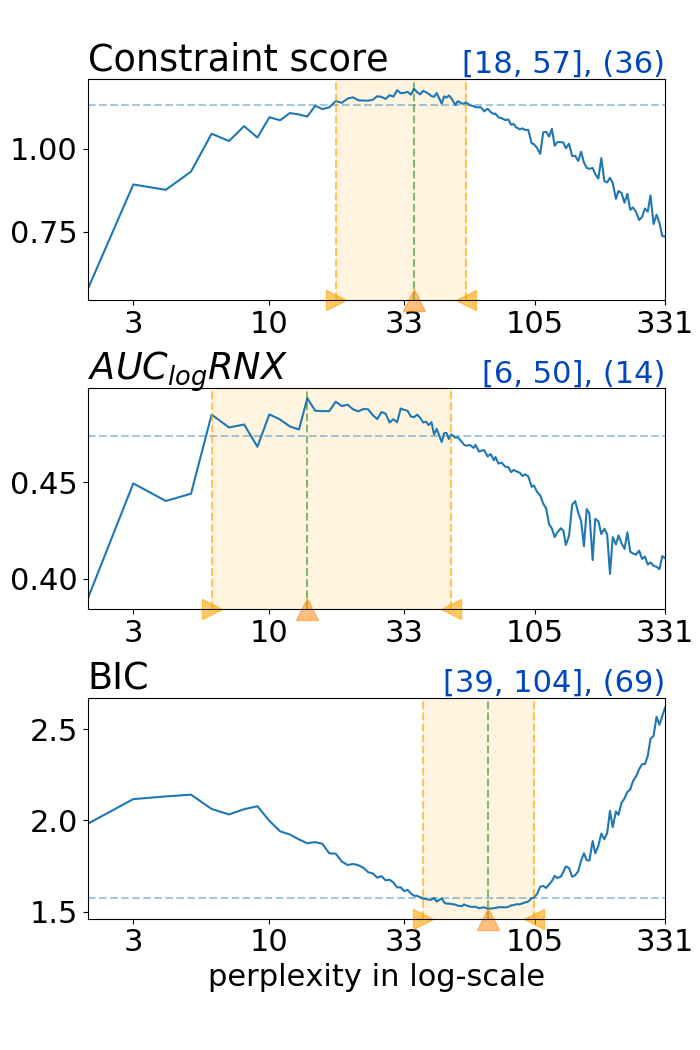
\includegraphics[width=\linewidth]{FASHION1000_tsne_compare_scores}
        \caption{FASHION\_1K}
    \end{subfigure}
    ~
    \begin{subfigure}[b]{0.3\linewidth}
        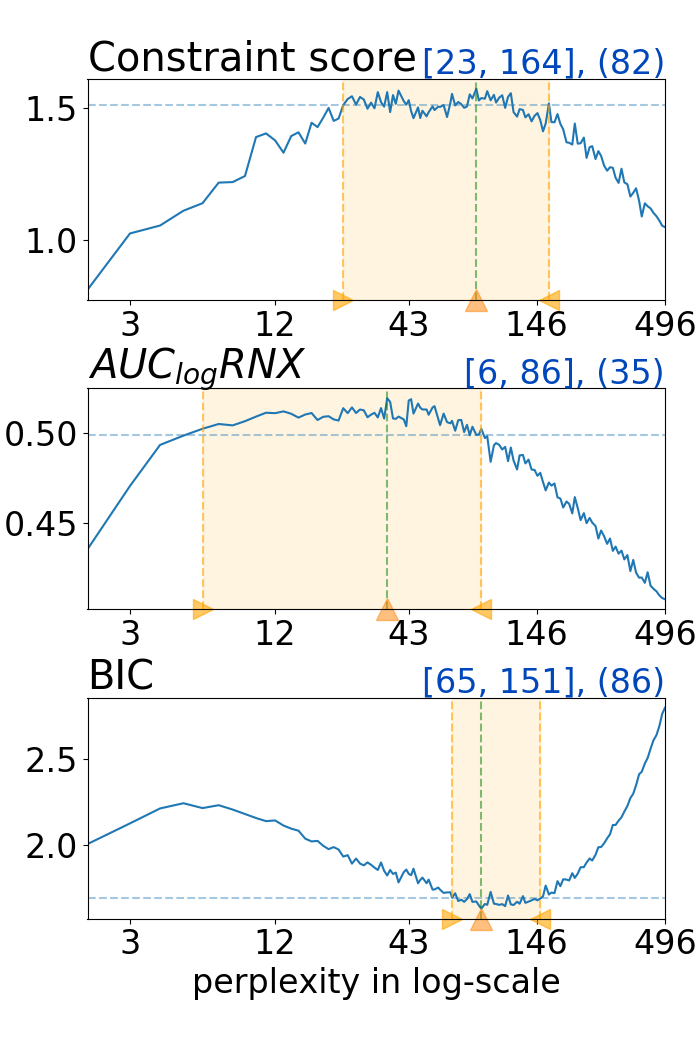
\includegraphics[width=\linewidth]{FASHION_MOBILENET_tsne_compare_scores}
        \caption{FASH\_MOBI}
    \end{subfigure}
    ~
    \begin{subfigure}[b]{0.3\linewidth}
        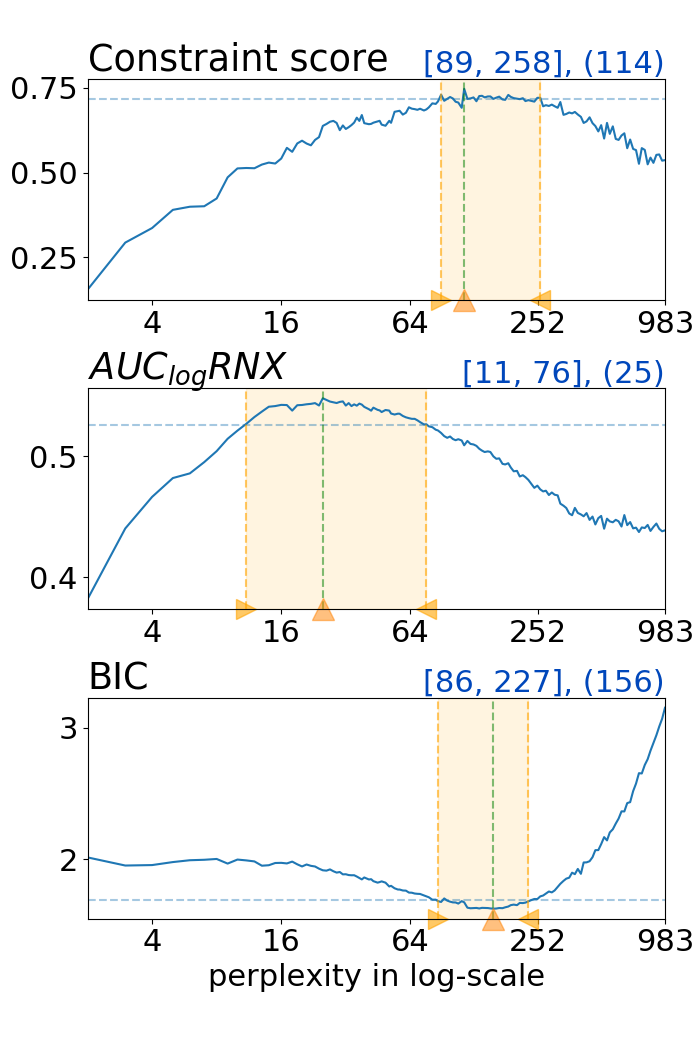
\includegraphics[width=\linewidth]{20NEWS5_tsne_compare_scores}
        \caption{5NEWS}
    \end{subfigure}
    \caption{Comparison of constraint score, $AUC_{log}RNX$ score and BIC score for $t$-SNE's embeddings.}
    \label{fig:tsne:compare}
\end{figure}
~
%% FIGURE metamap UMAP example
\begin{figure*}[ht!]
    \centering
    \begin{subfigure}[b]{.8\linewidth}
        \centering
        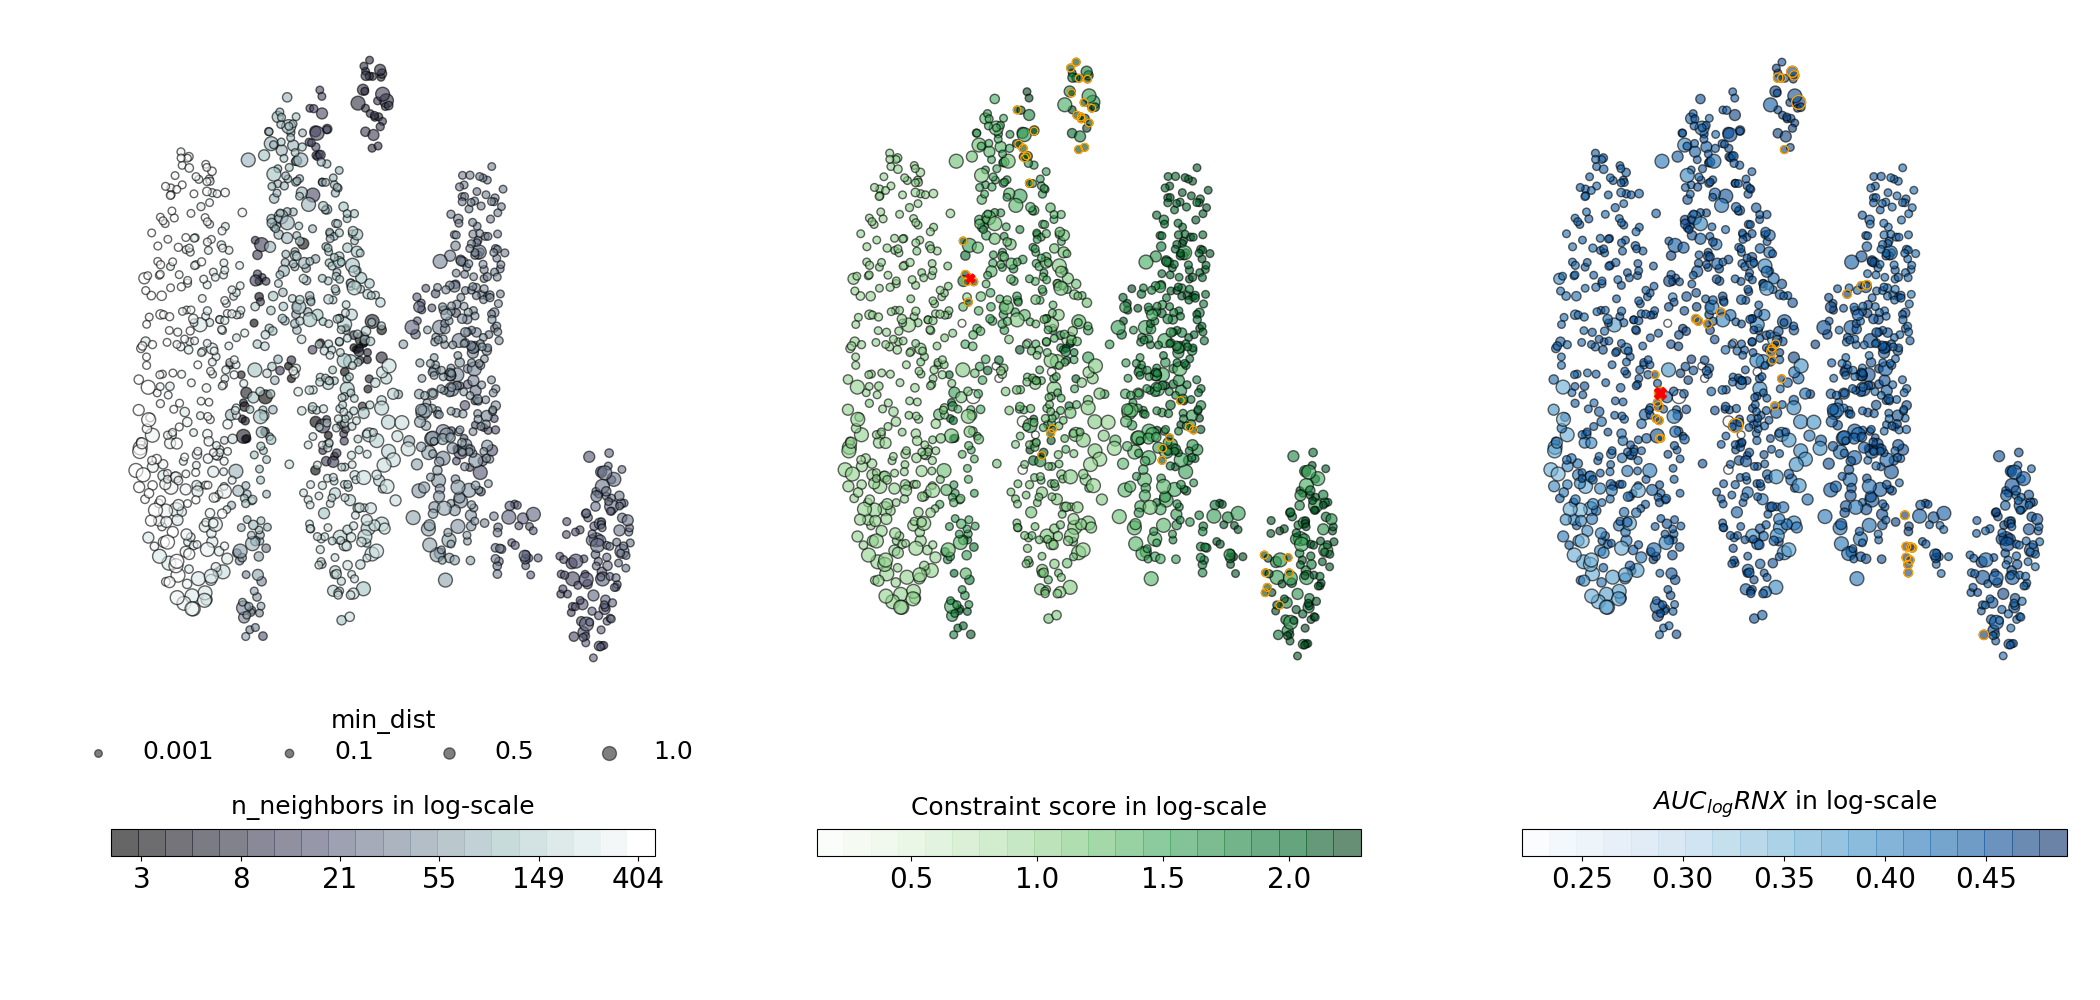
\includegraphics[width=\linewidth]{COIL20_umap_metamap}
    \end{subfigure}
    ~
    \begin{subfigure}[b]{.8\linewidth}
        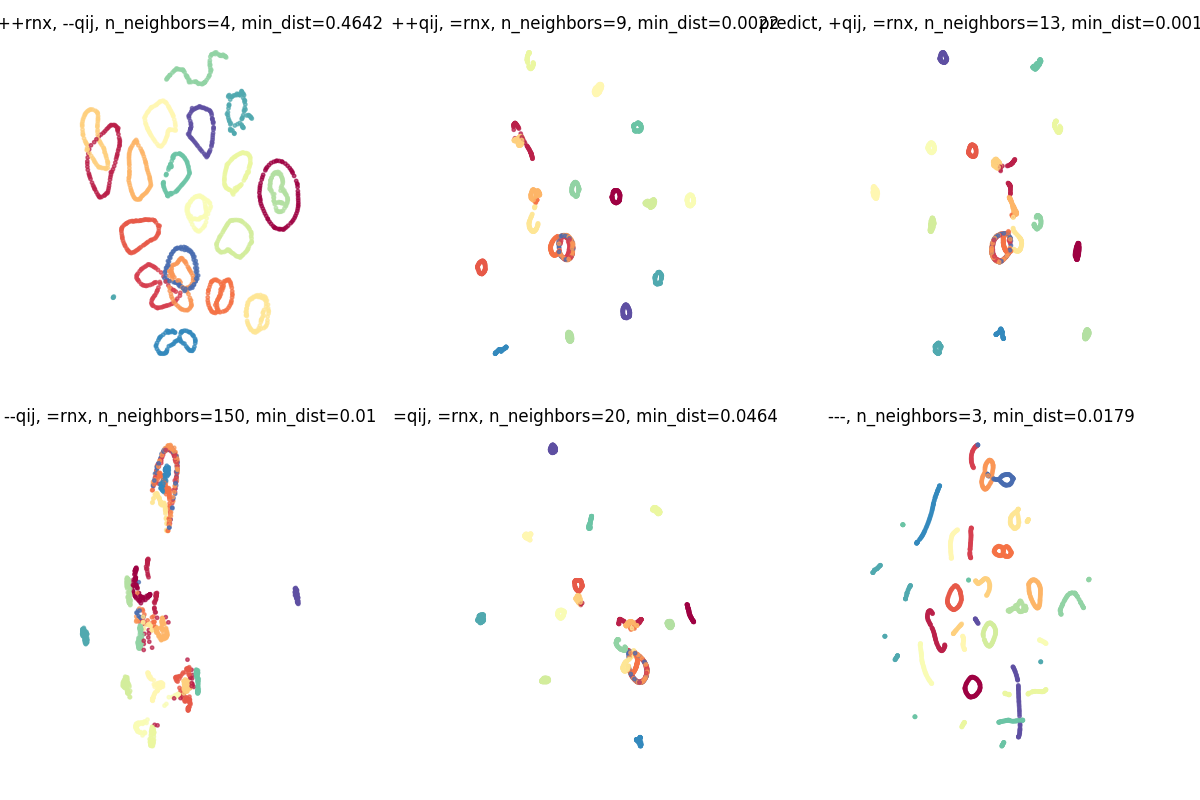
\includegraphics[width=\linewidth]{COIL20_umap_show}
    \end{subfigure}
    \caption{Metamaps and visualizations with hyperparameters by BayOpt based on $f_{score}$ for COIL20.}
    \label{fig:umap:meta:COIL20}
\end{figure*}
~
%% FIGURE compare 2 scores UMAP
\begin{figure}[ht!]
    \centering
    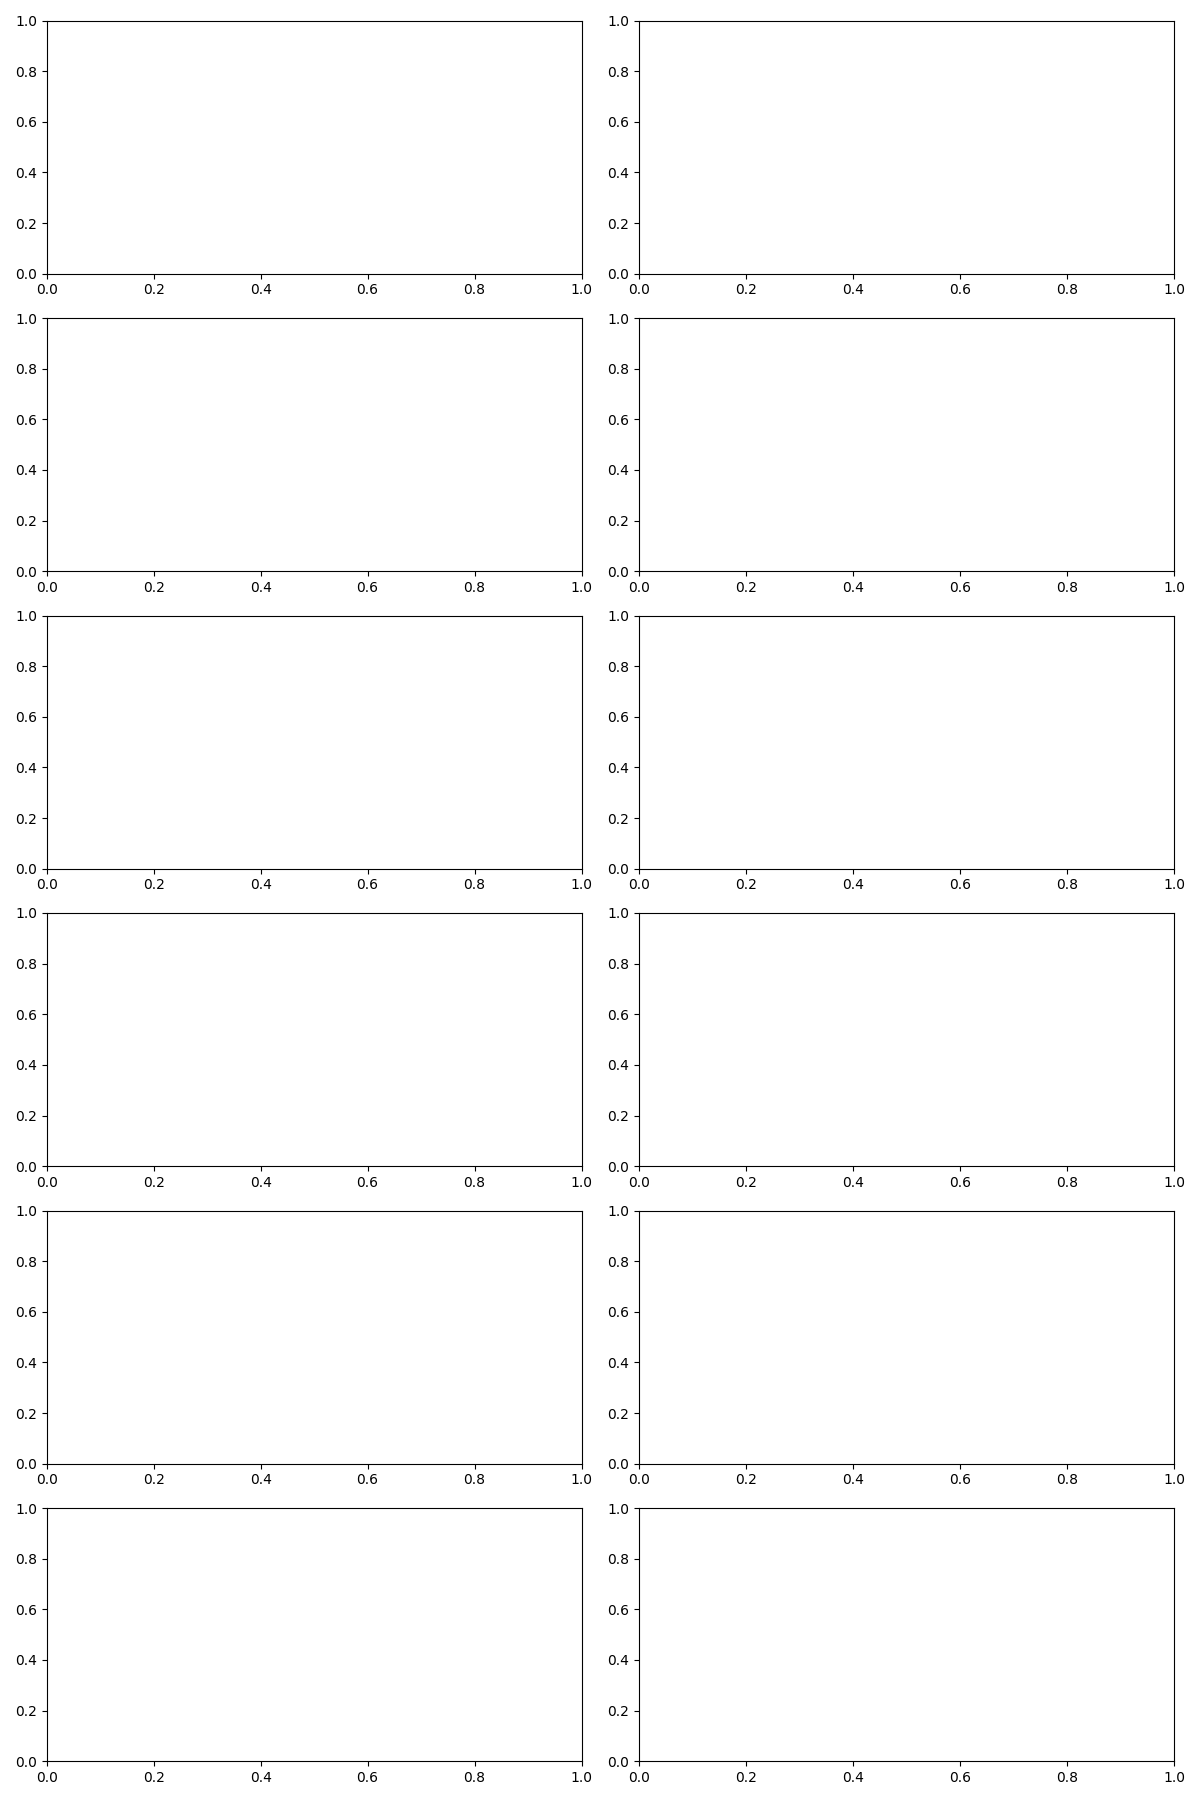
\includegraphics[width=.8\linewidth]{umap2D_compare}
    \caption{Compare $f_{score}$ and $AUC_{log}RNX$ for UMAP embeddings.}
    \label{fig:score:umap2D:compare}
\end{figure}


$f_{score}$ is compared with $AUC_{log}RNX$ and BIC-based score for evaluating $t$-SNE embeddings in Section~\ref{sec:compare:tnse}.
It is compared with $AUC_{log}RNX$ for evaluating UMAP embeddings in Section~\ref{sec:compare:umap}.
% In all comparison, $f_{score}$ is calculated from the constraints generated by 10 labeled instances per class on each dataset.

\subsection{Compare $f_{score}$, $AUC_{log}RNX$ and BIC-based score for $t$-SNE}\label{sec:compare:tnse}

Fig.~\ref{fig:tsne:compare} illustrates the best perplexity ranges found by $f_{score}$, $AUC_{log}RNX$ and the BIC-based score for the six selected datasets.
$f_{score}$ agrees with both $AUC_{log}RNX$ and the BIC-based score for COIL20 and {FASH\_MOBI} datasets.
$f_{score}$ agrees only with $AUC_{log}RNX$, but not the BIC-based score for {FASHION\_1K} dataset.
Moreover, $f_{score}$ agrees only with the BIC-based score, but not $AUC_{log}RNX$, for {NEURON\_1K}, 5NEWS and DIGITS datasets.
In order to compare thoroughly the best solutions found by these three scores, metamaps can be used.

A metamap is used to visualize the solution space of a DR visualization, i.e., to represent embeddings with different perplexities on a 2D space.
Each point in this metamap is an embedding corresponding to one perplexity, meaning that two points close together correspond to perplexities that provide similar visualizations.
The metamaps presented in this section contains points that are $t$-SNE visualizations, and are built by UMAP with {n\_neighbors} = 50 and {min\_dist} = 0.1.
UMAP with large {n\_neighbors} is used to build the metamap in order to obtain an overall view about the global relation of all embeddings.
% UMAP is used to build the metamap because of its capacity to consider the overall view, in addition to its focus on neighborhoods.
% Indeed, the large value of {n\_neighbors} (50) is used to obtain an overall view about the global relation of all embeddings.

In Fig.~\ref{fig:tsne:meta:NEURON1K}, some selected perplexity values are highlighted in the metamaps for {NEURON\_1K} dataset, and the corresponding visualizations are shown below them.
The four metamaps are colored by the values of perplexity, $f_{score}$, $AUC_{log}RNX$ and the BIC-based score respectively.
The embeddings with the highest score (superior than 96\% of maximum score) are highlighted.
For the real world {NEURON\_1K} dataset, the three scores discover different regions in the solution space. This can help the user to observe the structure of the dataset under different aspects given by the different quality scores.

The visualizations at the bottom of Fig.~\ref{fig:tsne:meta:NEURON1K} served as a qualitative evaluation of the best visualizations found by $f_{score}$, $AUC_{log}RNX$ and the BIC-based score.
The ranks used for the scores are: very preferred ($\Uparrow\Uparrow$), preferred ($\Uparrow$), good enough ($[]$), not preferred ($\Downarrow$) and unfavorable ($\Downarrow\Downarrow$).
The visualization that is best predicted by BayOpt is denoted by a star symbol ($\star$).
As indicated by Wattenberg et. al.~\cite{wattenberg2016use}, more than one visualization may be needed to understand the high-dimensional patterns in the data.
The visualizations extracted thanks to the different scores make it easier to discover different regions in the solution space, and thus to discover different structures in the data, while one score could not reveal them all.

\subsection{Compare $f_{score}$ and $AUC_{log}RNX$ for UMAP}\label{sec:compare:umap}

A two dimensional grid of {n\_neighbors} and {min\_dist} hyperparameters is created to evaluate $f_{score}$ and $AUC_{log}RNX$ for the UMAP embeddings of all six datasets.
% The values of these two scores are shown in the contour plots in Fig.~\ref{fig:score:umap2D:compare}.
% {n\_neighbors} plays the same role as the perplexity of $t$-SNE and LargeVis.
% It controls how large structures in the data should be conserved and affects the construction of the k-neighbor graph in HD.
% A small value leads to many small connected components in the visualization, while a large value provides a boarder view of the data.
% A suggested range for {n\_neighbors} is $[5, 50]$.
% {min\_dist} in its turn, affects directly the output since it controls how tightly points are packed together. It is considered to be most important hyperparameter for UMAP \cite{mcinnes2018umap}.
% The recommended range for {min\_dist} is $[0.001, 0.5]$.
For the three simple datasets (DIGITS, COIL20 and {FASHION\_1K}), $f_{score}$ shows clearly the evolution of the score value in comparison to $AUC_{log}RNX$.
For {NEURON\_1K} dataset, the two score discover different optimal zones but with the same principle.
For the two other datasets ({FASH\_MOBI} and 5NEWS), $AUC_{log}RNX$ shows clearer the zones of the best hyperparameters.
However, in general, the contour plots of $AUC_{log}RNX$ suggest that this score is not sensitive to the {min\_dist} hyperparameter.
Indeed, with a fixed value of {n\_neighbor}, it is likely that $AUC_{log}RNX$ gives the same score for different values of {min\_dist}.
In contrast, $f_{score}$ can discover the influence of {min\_dist} in conjunction with {n\_neighbor} and reveal a reasonable small zone for the best combination of these two hyperparameters.


As for $t$-SNE in Section~\ref{sec:result:bo:tsne}, metamaps of the different visualizations that can be generated by UMAP are presented at the top of Fig.~\ref{fig:umap:meta:COIL20}, and four different visualizations are selected and shown at the bottom of the figure.
The first visualization (bottom left of Fig.~\ref{fig:umap:meta:COIL20}) presents the visualization generated by UMAP with the best predicted combination of hyperparameter values, according to $f_{score}$.
The next two visualizations are considered good by $AUC_{log}RNX$, but not by $f_{score}$.
In the second visualization, several groups are overlapping. Since the points in same group are not close together, $f_{score}$ is smaller than for the first visualization.
The last visualization belongs to a region of points in the metamaps that have low values for both scores.
These regions are the ones that are never highlighted in the metamaps, which correspond to visualizations that have a too large {n\_neighbors} and/or a too large {min\_dist}. 

%%%%%%%%%%%%%%%%%%%%%%%%%%%%%%%%%%%%%%%%%%%%%%%%%%%%%%%%%%%%%%%%%%%%%%%%%%%%%%%%
\section{BayOpt for hyperparameter tuning with $f_{score}$}\label{sec:apply-bayopt}

Finding the best hyperparameters by greedily searching through the grid is not practical and scalable, but it is used in the experiment to compare with the BayOpt approach.
The BayOpt approach solves this scalability problem efficiently, in which only dozens of evaluations are required to find the best hyperparameters for all experimented datasets.

For the hyperparameter tuning task under BayOpt framework in this work, the exploration strategy is preferred to ensure to discover the largest as possible the parameter space.
Expected Improvement (EI) acquisition function is used as a surrogate function of BayOpt.
This function maximizes the expected improvement over the current best parameters and proves its efficiency in practice~\cite{snoek2012practical}.
In EI, the parameter $\xi$ controls the trade-off between global search (exploration) and local optimization (exploitation).
$\xi$ is set to a large value (0.1) to realized the exploration strategy, that works well for all experimented dataset without any effort to tune this parameter.
Since there is always a small variance in the score value, 
the input observations (the $f_{score}$ values) for BayOpt can be corrupted by noise.
Small values are added to the diagonal of the kernel function of the underlying Gaussian Process model to handle this noise.


As empirically proved in the previous sections, $f_{score}$ is a reliable score to evaluate the quality of the embeddings.
BayOpt is widely used for hyperparameter tuning, when the target function is well-defined and assures to find global maximum of a well-formed function like $f_{score}$.
In Section~\ref{sec:result:bo:tsne} and Section~\ref{sec:result:bo:umap}, $f_{score}$ is evaluated for the tasks of tuning one hyperparameter under BayOpt framework for $t$-SNE two hyperparameters for UMAP, respectively.
% However naive search through the grid of hyperparameters is exponentially expensive when the number of hyperparameters increases.
% BayOpt helps to explore the parameter spaces efficiently and focus the computation only on the zones of potential parameters which give high values for the target function.
% It is widely used for hyperparameter tuning, when the target function is well-defined and assures to find global maximum of a well-formed function like $f_{score}$.
% $AUC_{log}RNX$ score or the BIC-based score can be used as a target function in BayOpt.
% However, our experiments show that $AUC_{log}RNX$ does not always work well with UMAP's embedding, especially in the case of tuning two UMAP's hyperparameters at the same time.
% The BIC-based score, by definition, is tied to $t$-SNE and does not work for other DR methods.
% $f_{score}$ is designed to be independent to the DR methods and to be flexible to the input constraints.
% In this section, the input constraints are generated from 10 labeled instances per class for any given dataset.
% $f_{score}$, which is flexible by design, can find the best visualization w.r.t. any set of input constraints.
% This task can not be achieved neither by $AUC_{log}RNX$ nor by BIC-based score.

\subsubsection{BayOpt for Tuning One Parameter of $t$-SNE}\label{sec:result:bo:tsne}

%% FIGURE BO tSNE
\begin{figure}[ht!]
    \begin{subfigure}[b]{.46\linewidth}
        \centering
        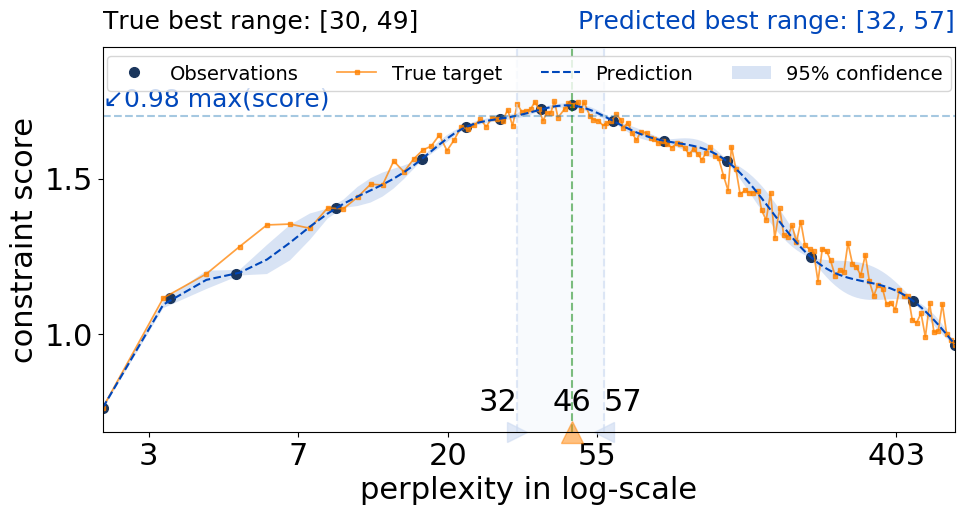
\includegraphics[width=\linewidth]{DIGITS_tsne_bo.png}
        \caption{DIGITS}
    \end{subfigure}
    ~
    \begin{subfigure}[b]{.46\linewidth}
        \centering
        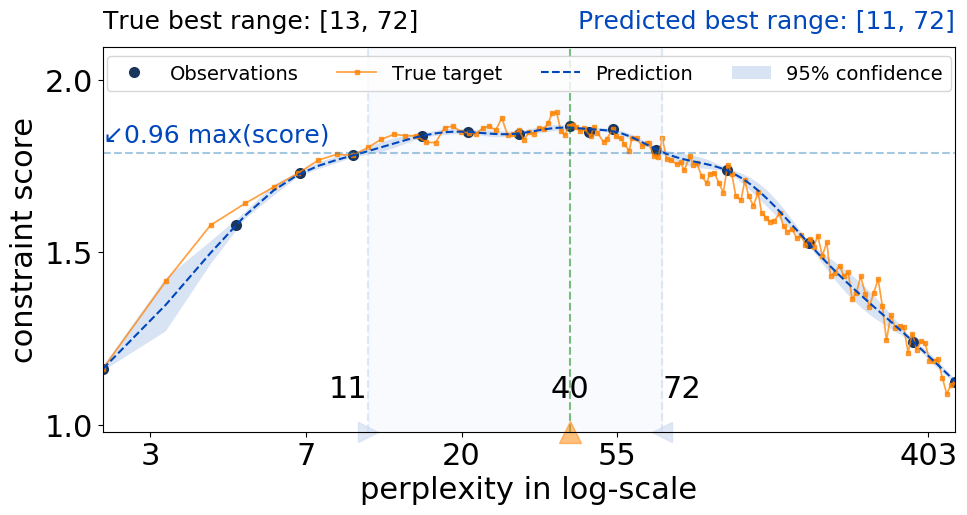
\includegraphics[width=\linewidth]{COIL20_tsne_bo.png}
        \caption{COIL20}
    \end{subfigure}
    \vfill
    \begin{subfigure}[b]{.46\linewidth}
        \centering
        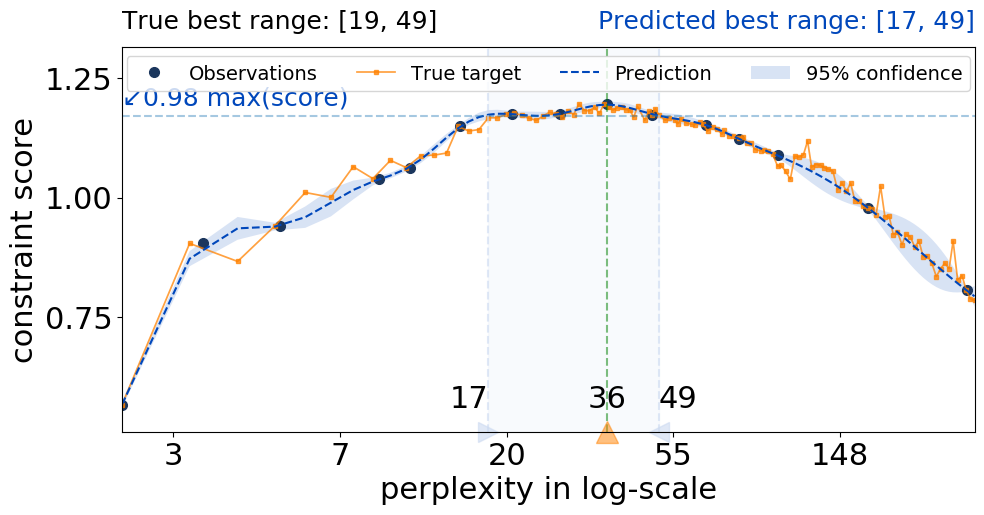
\includegraphics[width=\linewidth]{FASHION1000_tsne_bo.png}
        \caption{{FASHION\_1K}}
    \end{subfigure}
    ~
    \begin{subfigure}[b]{.46\linewidth}
        \centering
        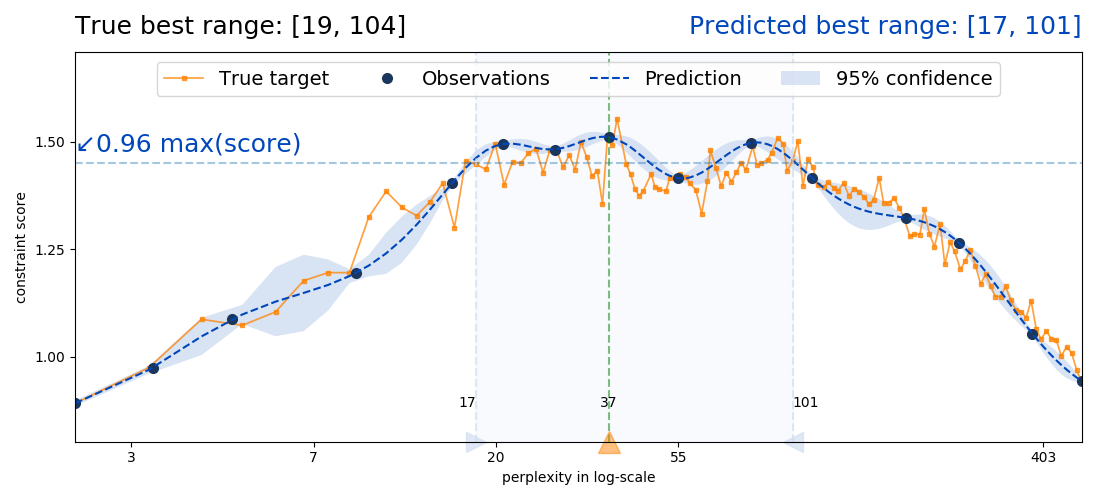
\includegraphics[width=\linewidth]{FASHION_MOBILENET_tsne_bo.png}
        \caption{{FASH\_MOBI}}
    \end{subfigure}
    ~
    \vfill
    \begin{subfigure}[b]{.46\linewidth}
        \centering
        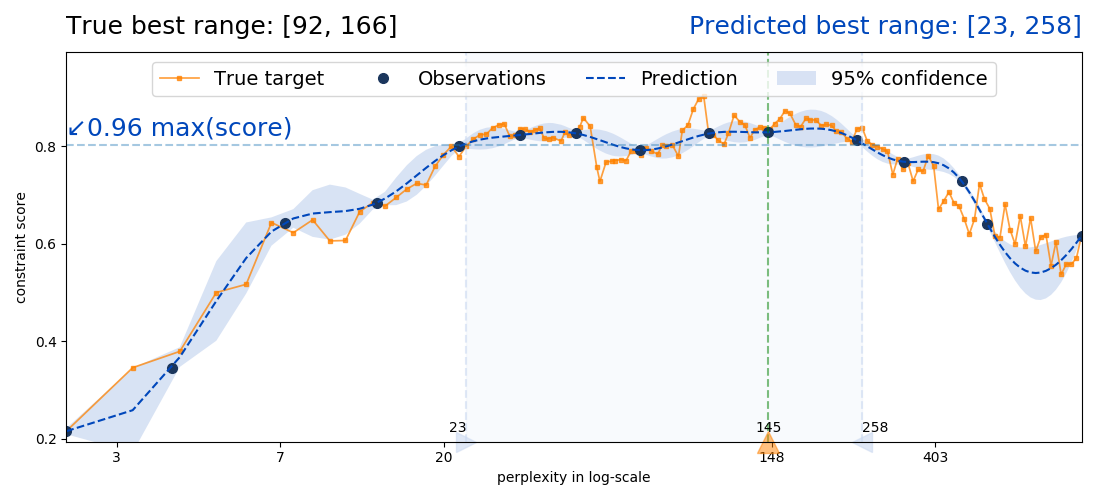
\includegraphics[width=\linewidth]{20NEWS5_tsne_bo.png}
        \caption{5NEWS}
    \end{subfigure}
    ~
    \begin{subfigure}[b]{.46\linewidth}
        \centering
        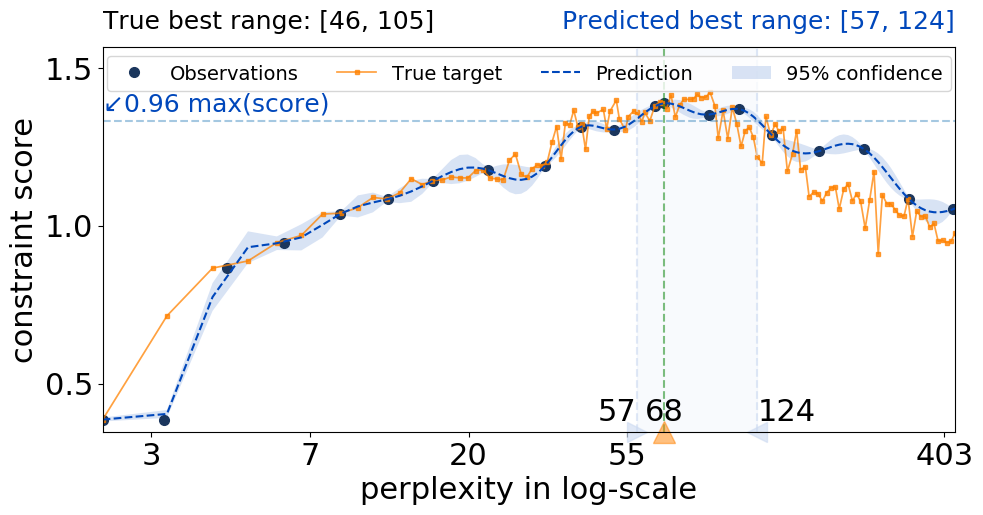
\includegraphics[width=\linewidth]{NEURON_1K_tsne_bo.png}
        \caption{{NEURON\_1K}}
    \end{subfigure}
    \caption{BayOpt approach for  $t$-SNE}
    \label{fig:tsne:bo:all}
\end{figure}

Fig.~\ref{fig:tsne:bo:all} demonstrates how BayOpt works for tuning $t$-SNE's perplexity for all six selected datasets.
% As shown empirically in the previous section, 10 labeled instances for each class suffice for a stable score.
% The scores are calculated for all sampled perplexity values $\in [2, N/3]$, with $N$ being the number of instances in the dataset.
For all datasets of various sizes (from 1000 to around 3000 instances), the scores needs to be evaluated for only 15 selected perplexities.
% These perplexity values are selected by BayOpt iteratively, starting with five perplexities randomly initialized.
% The score for each perplexity $p_i$ is calculated and all pairs $\{p_i, f_{score}(p_i)\}$ are used to train the BayOpt model.
% The next predicted perplexity to evaluate is the most promising value according to the BayOpt model.
% When the new perplexity is evaluated, BayOpt gets the new score value and update its model.
% More detail and visual explanation on how BayOpt works with the proposed score function can be found in \ref{app:bo:explain}.
It should be noted that BayOpt does not approximate the score function, but tries to find its maximum value instead.
% Fig.~\ref{fig:tsne:bo:all} shows the prediction of the best perplexity for BayOpt on each dataset, with a convergence after only 15 iterations.
The best predicted perplexity range (in which the predicted score is superior to 96\% of the maximum predicted score) is highlighted in the vertical region.
BayOpt does not only find the best hyperparameter values, but also indicate the region in which it is not certain about its prediction.
This is usually the region of high perplexity values, where the $f_{score}$ has large distortions.

\subsubsection{BayOpt for Tuning Two Parameters of UMAP}\label{sec:result:bo:umap}

%% FIGURE BO UMAP
\begin{figure}[ht!]
    \begin{subfigure}[b]{.48\linewidth}
        \centering
        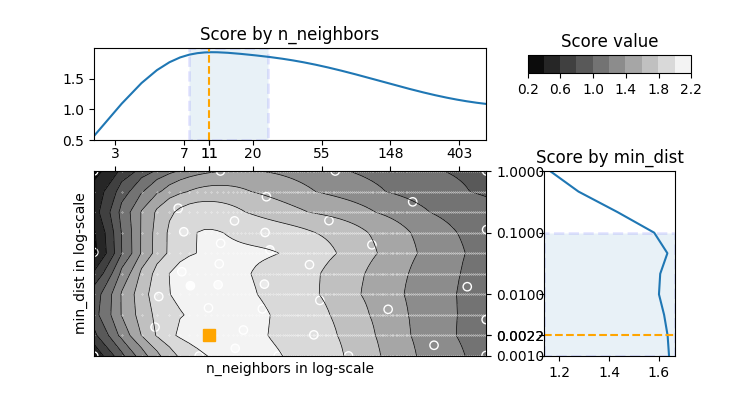
\includegraphics[width=\linewidth]{DIGITS_umap_predicted_score}
        \caption{DIGITS}
        \label{fig:bo:umap:predict:DIGITS}
    \end{subfigure}
    ~
    \begin{subfigure}[b]{.48\linewidth}
        \centering
        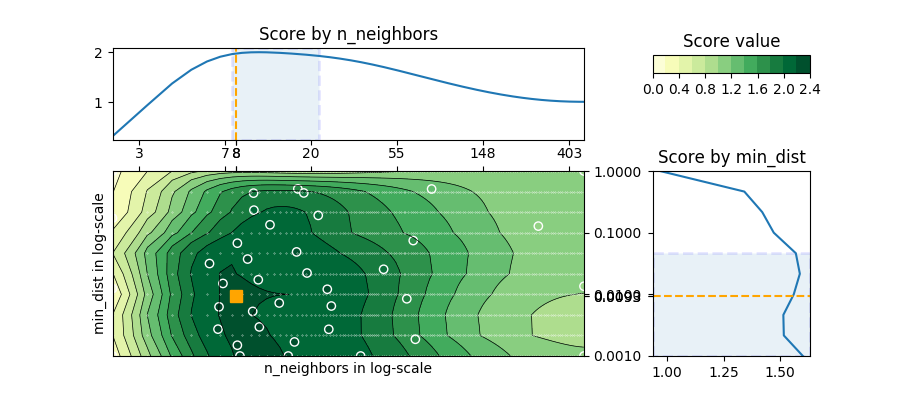
\includegraphics[width=\linewidth]{COIL20_umap_predicted_score}
        \caption{COIL20}
        \label{fig:bo:umap:predict:COIL20}
    \end{subfigure}
    \vfill
    \begin{subfigure}[b]{.48\linewidth}
        \centering
        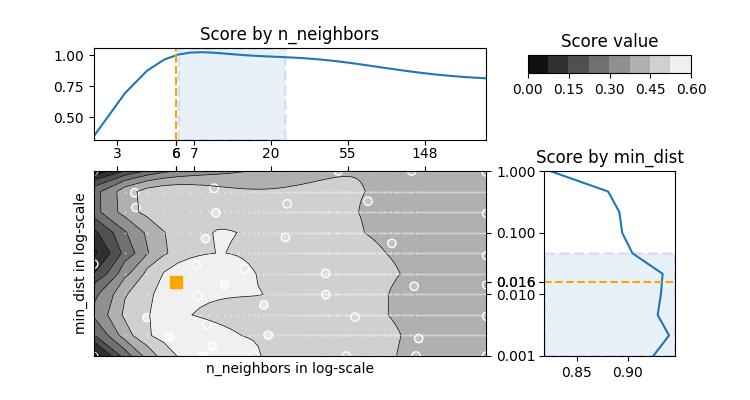
\includegraphics[width=\linewidth]{FASHION1000_umap_predicted_score}
        \caption{{FASHION\_1K}}
        \label{fig:bo:umap:predict:FASHION1K}
    \end{subfigure}
    ~
    \begin{subfigure}[b]{.48\linewidth}
        \centering
        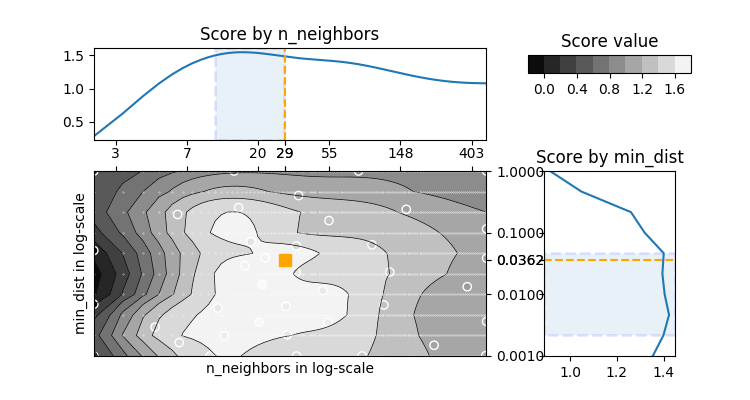
\includegraphics[width=\linewidth]{FASHION_MOBILENET_umap_predicted_score}
        \caption{{FASH\_MOBI}}
        \label{fig:bo:umap:predict:FASHMOBI}
    \end{subfigure}
    \vfill
    \begin{subfigure}[b]{.48\linewidth}
        \centering
        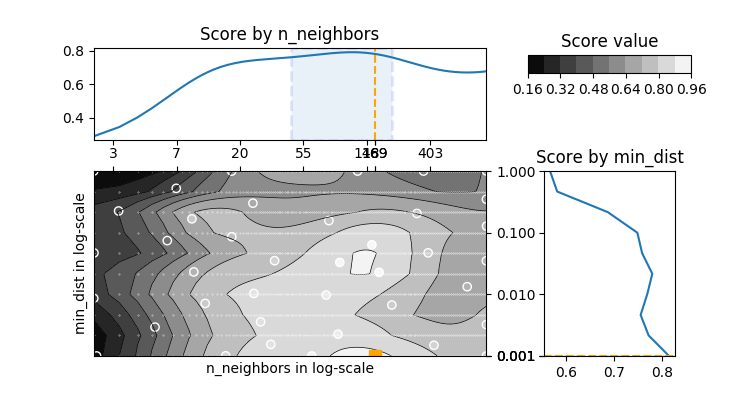
\includegraphics[width=\linewidth]{20NEWS5_umap_predicted_score}
        \caption{5NEWS}
        \label{fig:bo:umap:predict:5NEWS}
    \end{subfigure}
    ~
    \begin{subfigure}[b]{.48\linewidth}
        \centering
        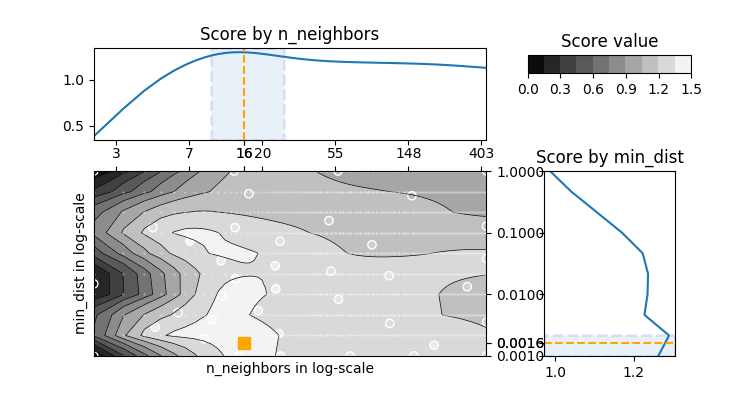
\includegraphics[width=\linewidth]{NEURON_1K_umap_predicted_score}
        \caption{{NEURON\_1K}}
        \label{fig:bo:umap:predict:NEURON1K}
    \end{subfigure}
    \caption{BayOpt for tuning the two hyperparameters of UMAP for all datasets.}
    \label{fig:bo:umap:predict}
\end{figure}

Tuning hyperparameters for UMAP is more difficult since the parameter grid is much larger than one of $t$-SNE.
Instead of evaluating thousands of combinations of two hyperparameters, BayOpt converges only after 40 iterations for all six experimented datasets.
Fig.~\ref{fig:bo:umap:predict} demonstrates how BayOpt works to find the zone of best combinations for the six datasets.
The uncertainty of BayOpt prediction is not shown in this plot.
In comparison with the fully evaluated grid of $f_{score}$ in Fig.~\ref{fig:score:umap2D:compare},
it is clear that BayOpt can approximate the zone of highest score efficiently with a very limited number of evaluation.

In practice, BayOpt is used to tune an ensemble of multiple hyperparameters.
The contour plots of every pair of hyperparameters are always used to investigate the zone of best combinations.
One main advantage of BayOpt approach is that, it does not only maximize the target score function but also give an estimated score prediction for all parameter combinations.
Indeed, in each plot in Fig.~\ref{fig:bo:umap:predict}, there are only 40 points that are exactly evaluated.
The contour is built upon the predicted value of the BayOpt's underlying Gaussian Process model for all other points.
Without spending much resource to obtain a full grid, the estimated score given by BayOpt is reliable enough to point out the best hyperparameters.


%%%%%%%%%%%%%%%%%%%%%%%%%%%%%%%%%%%%%%%%%%%%%%%%%%%%%%%%%%%%%%%%%%%%%%%%%%%%%%%%
\section{Discussion}\label{sec:discussion}
$t$-SNE, LargeVis and UMAP are widely used since they produce reasonable visualizations.
Despite of their power, it is always necessary to tune their hyperparameters for a particular given dataset.
This work presents a solution for tuning hyperparameters of these methods by introducing the constraint preserving $f_{score}$.
In this section, we discuss the specific use of BayOpt for optimizing $f_{score}$, the flexibility and computational efficiency of this score.


\subsection{Why using BayOpt for $f_{score}$?}
The proposed $f_{score}$ has an advantage in its flexibility, but the score value is not deterministic.
With the same number of labeled instances or the same number of constraints, the score may vary w.r.t. chosen sets of constraint pairs.
BayOpt approach fits well in this situation, since it can learn from noisy observation.
The underlying predictive model of the BayOpt framework is a Gaussian process (GP) model.
In the context of our work, the GP model is based on the assumption that similar hyperparameter values give similar embeddings, and thus similar output score values.
In practice, we found that this assumption is true for all three selected DR methods and all experimented datasets.

The well-formed $f_{score}$ function help BayOpt estimate correctly its global maximum.
BayOpt also converges quickly thanks to the exploration strategy combining with the parameters sampled in log-scale.
% that helps discover the good range of parameters and eliminate the range of too small or too large values.
% In our problem, there is a major reason why the prediction of BayOpt converges quickly to the global optimum (after 15 iterations for tuning $t$-SNE's perplexity and 40 iterations for tuning UMAP's two hyperparameters): the proposed score function is well-formed, which makes it very simple to find its maximum.
% Second, the exploration strategy used in BayOpt's Expected Improvement acquisition function, combining with the parameters sampled in log-scale helps us quickly discover the good range of parameters and eliminate the range of too small or too large values. (See the density of evaluated points in Fig~\ref{fig:tsne:bo:all} and Fig~\ref{fig:bo:umap:COIL20:prediction}).
Moreover, the iterative predictions of BayOpt are visible, which makes the optimization explainable for non-expert users.
Indeed, BayOpt can be run iteratively to investigate why a particular hyperparameter value is chosen, or to directly guide the optimization process. For instance, the user can specify the hyperparameter to evaluate and the GP model will update itself to learn from both the already evaluated $f_{score}$ and the new probed observation.

\subsection{$f_{score}$ is a Flexible Function}
All three examined DR methods preserve well the neighborhood information.
However $t$-SNE does not guarantee to preserve the overall distance and much global structure in the data.
UMAP is presented to preserve more global structure with the cost of tuning more hyperparameter.
The users can look for a global structure (a hierarchical or semantic grouping) or another view to discover different structures.
This goal can be easily encoded in term of labeled instances and transformed into pairwise constraints for the proposed $f_{score}$.
It has been shown in our experiments that such a specific, desired structure may exist in the solution space of $t$-SNE embeddings, but $AUC_{log}RNX$ or the BIC-based score could not reveal.
$f_{score}$, in addition to be a reliable method to tune DR hyperparameters, is also a flexible score that can reveal a specific, desired desired global structure by users.

Unlike $AUC_{log}RNX$ or the BIC-based score, which do not depend on external input data, $f_{score}$ is a function of a given ensemble of similar-link constraints $\mathcal{S}$ and dissimilar-link constraints $\mathcal{D}$.
$AUC_{log}RNX$ objectively measures how neighborhoods are preserved without taking into account the interest of users.
As demonstrated in Section~\ref{sec:result:flexibility} with three real world datasets, $f_{score}$ can discover solutions satisfying users' constraints that are never selected by $AUC_{log}RNX$ nor the BIC-based score.

Moreover, the constraint score function can be easily modified to adapt to different criteria, such as the contrastive measure or the triplet measure.
These are adapted version based on the idea of contrastive loss~\cite{logeswaran2018efficient} and triplet loss~\cite{schroff2015facenet}, which use several selected anchor points, their positive examples (connected by similar-links) and their negative examples (connected by dissimilar-links).
% $\mathbb{E}_{y, y_+, y_-} \Big[ -\log \Big( \frac{exp(y^T y_+)}{exp(y^T y_+) + exp(y^T y_-)} \Big) \Big]$
% $\mathbb{E}_{y, y_+, y_-} \Big[ max(0, ||y-y_+||^2 - ||y-y_-||^2  \Big]$

%%%%%%%%%%%%%%%%%%%%%%%%%%%%%%%%%%%%%%%%%%%%%%%%%%%%%%%%%%%%%%%%%%%%%%%%%%%%%%%%
\section{Conclusion and Future Work}\label{sec:conclusion}
\todo[inline]{Latter}

The principle contribution of this work is to propose a flexible constraint preserving score to quantitative measure the quality of any DR methods.
This score is used in a Bayesian Optimization framework to find the best visualization of $t$-SNE, LargeVis and UMAP.
The proposed constraint-based score is independent to how the embedding is produced and can be used with any DR methods.
This score is built upon a limited number of constraints but can distinguish the visualizations preferring local structure and those preferring global structure.
A finding that Bayesian Optimization approach fits well in our problem.

The constraint-based score agree the the well-known quality metric.
This score can be visually represented to explain the violated pairs.
By combining this score with BayOpt approach, we can tune many hyperparameters at the same time for many widely used DR methods like $t$-SNE or UMAP.
BayOpt takes into account the uncertainty in the score values and also explainable. We can observe the internal optimization step to answer the question: why to choose the next promising hyperparameters to try?
The hyperparameters of $t$-SNE and UMAP make these methods difficult to use correctly but also make them flexible.
These methods can produce different visualizations and reveal different hidden structures in the data.
To evaluate the embedding quality of such flexible methods, we need a flexible score.
The state of the art $AUC_{log}RNX$ metric or the BIC-based score has no flexibility to capture different visualization results.

Future work: User experiment:
The constraint generation can be guided by the users and the visualization quality can be evaluated by them.
Since the proposed constraint score proved to be stable w.r.t the number of labeled instances,
we can use the user-defined labeled instances to generate the pairwise constraints.
As demonstrated with the labeled instances of three different groups characterized by UMI count in \emph{NEURAL\_1K} dataset, the users can define their need about the structure they look for.
A potential future work is to let the users evaluate qualitatively the quality of the visualization and their satisfaction.
Integrate the user's feedback in two stages of our workflow.
The users can select the pairwise constraints or label some points (used to generate the constraints) to build the score.
They can also manually select the next hyperparameters to evaluate in a customized interactive BayOpt framework.
Take the preference of the users on the presented visualizations to evaluate the quality of the visualization. We search for if the best visualization selected by the user corresponds to the result of our method.
